\section{Introduction}\label{section-introduction}

%$\alpha\beta\gamma\delta\epsilon\varepsilon\zeta\eta\theta\rho\varrho$
%$<\leq\geq>\subset\supset\supseteq\subseteq\pm\mp\times\div\ast\star\circ\cdot$

Hierarchical structures (or trees) frequently occur in information management that required to be stored and retrieved. Common examples of such structure include organization chart, in which positions of an organization are displayed as a tree, and hierarchical file system where files are stored in levels of directories.

Due to the popularity of relational database management systems (RDBMS), it is often required to store hierarchy data in such databases. The first apparent question is how to store hierarchical data in tables of RDMBS, which are great for storing a list of items without much design foresight for storing hierarchical data?

This paper explores ways of storing hierarchical data in relational databases. The goal is to define a few common operations of hierarchical data, the issues of implementing tree structure in relational model, and optimization for these operations.

\section{Definition}\label{section-definition}

\subsection{Tree}\label{section-tree}

Hierarchical data structure is also known as a tree, which is defined as a connected acyclic digraph $G=(V,E)$ of a set of vertices $V$ (also called nodes) and a set of edges $E$ that denotes the relationship between two nodes\footnote{https://en.wikipedia.org/wiki/Tree\_(data\_structure)}. Figure~\ref{fig:tree} depicts a typical tree.

\begin{figure}[!h]
\begin{center}
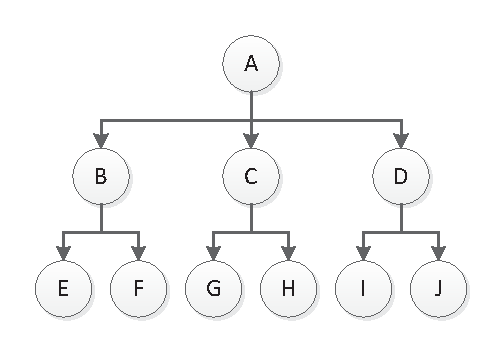
\includegraphics[width=2in]{images/tree.eps}
\caption{Example of a tree.\label{fig:tree}}
\end{center}
\end{figure}

Each node of the tree can hold any number of data item. In the figure above, only identifiers (A--J) of the nodes are shown for simplicity of illustration. The edges of the tree between two nodes are often named children (and sometimes parent) relationship. The relationship is often non-symmetric (as in digraph); for example, $B$ is a child of $A$, but the reverse is not true.

In many literatures of computer data structures, the edges are defined as `children of' a node. For example, node $A$ has children $B$, $C$, and $D$. In the sense of relational database, it does not matter if the edges are defined as `children of' or `parent of'; when one is defined, the other is usually inherited, especially when indexes are used on the relational table in which the tree is stored. The relationship, therefore, will be left for the design of database schema.

\subsection{Relational Database}

Relational data model is proposed by Edgar Codd in 1970\cite{DBLP:journals/cacm/Codd70}. In this model, a database consists of a set of tables (also known as relations), which each consists of a set of tuples. In colloquial usage, tuples are also called records.

Figure~\ref{fig:relational_database} illustrates a relational database with 2 tables, each 3 attributes. The teachers table has 4 records (tuples) and the Courses table has 6.

\begin{figure}[!h]
\centering
\subfigure[Teachers Table]{
\label{tab:sample_data_a}
  \begin{tabular}{|c|c|c|}
  \hline
  {\bf ID} & {\bf Name} & {\bf Office} \\ \hline\hline
  1 & James Madison & A\\
  2 & John Adams & B\\
  3 & Ronald Reagan & C\\
  4 & Franklin Pierce & D\\
  \hline
  \end{tabular}}
\subfigure[Courses Table]{
\label{tab:sample_data_a}
  \begin{tabular}{|c|c|c|}
  \hline
  {\bf ID} & {\bf Name} & {\bf Teacher} \\ \hline\hline
  1 & Data Structures & 1\\
  2 & Intro to Algorithms & 1\\
  3 & Software Construction & 2\\
  4 & Computer Networks & 3\\
  5 & Operating Systems & 4\\
  6 & Compilers & 2\\
  \hline
  \end{tabular}}
\caption{A Relational Database\label{fig:relational_database}}
\end{figure}

\subsection{Common Tree Operations}\label{sec_tree_ops}

In this section, we define common operations on trees. We only define data reading operations due to the fact that these operations are the most commonly performed operations in database system after the initial insertion of data. Modification and deletion are less common and are usually trivial cases (compared to a myriad of important reading operations) to correct small mistakes. In addition, before updating or deletion, reading must be performed to locate the correct data to modify. With respect to hierarchical data, once an hierarchy is inserted into a database, the structure is rarely changed without removing an entire subtree.

We define the operations in this section without considering how the trees are implemented in relational model. Section \ref{sec-nested-set} and \ref{sec-adj-list} will cover implementation details and how these operations can be evaluated under a relational designs.

%This section only defines reading operations due to the fact that reading is more interesting. When modifying or deleting . There are more reading operations and unlike insertion and deletion, the performance of reading operations can be improved based on the careful design of the relational model. , relying on the assumption that once an hierarchy is inserted into a database, the structure is rarely changed without removing an entire subtree. Insertion operations are assumed to be done via standard SQL insert statements. Hierarchical update and remove operations are to be covered in future works.

Operations thtat will be used in this paper are enumerated below. All examples use the tree of Figure~\ref{fig:tree}.


%%% Enumeration of operations %%%

\begin{enumerate}

\item $Root(n) \rightarrow r$ : given a node $n$, this operation finds the root $r$ of the tree in which $n$ resides: $Member(n, r) \rightarrow true$.

    \begin{align*}
    & Root(A) \rightarrow A \\
    & Root(E) \rightarrow A
    \end{align*}

    
\item $Parent(n) \rightarrow p$ : Given a node $n$, this operation finds the parent node $p$, or $null$ if $n$ is a root node.

    \begin{align*}
    & Parent(A) \rightarrow  null \\
    & Parent(B) \rightarrow A
    \end{align*}

\item $Children(n) \rightarrow \{c_1, c_2, ..., c_n\}$ : Given a node $n$, this operation finds it's child nodes $\{c_1, c_2, ..., c_n\}$. If $n$ is a leaf node (no children), then the empty set is returned.

    \begin{align*}
    & Children(A) \rightarrow \{B, C, D\} \\
    & Children(E) \rightarrow \{\}
    \end{align*}
    
\item $Siblings(n) \rightarrow \{n_1, n_2, ..., n_n\}$ : This operation finds a list of nodes $\{n_1, n_2, ..., n_n\}$ that have the same depth as node $n$. If this node has no siblings, the empty set is returned.

    \begin{align*}
    & Siblings(A) \rightarrow \{\} \\
    & Siblings(B) \rightarrow \{C, D\}
    \end{align*}

\item $Leaves(n) \rightarrow \{n_1, n_2, ..., n_n\}$ : This operation returns a set of leaf nodes $\{n_1, n_2, ..., n_n\}$ of the subtree rooted at $n$

    \begin{align*}
    & Leaves(A) \rightarrow \{E, F, G, H, I, J\} \\
    & Leaves(B) \rightarrow \{E, F\} \\
    & Leaves(E) \rightarrow \{E\}
    \end{align*}
    
\item $Height(n) \rightarrow \mathbb{N}$ : Given a node $n$, this operation returns the count of node of longest path from $n$ to a leaf node.

    \begin{align*}
    & Height(A) \rightarrow 3 \\
    & Height(E) \rightarrow 1
    \end{align*}
    
\item $Depth(n) \rightarrow \mathbb{N}$ : Given a node $n$, this returns $|Path(n)|$.

    \begin{align*}
    & Depth(A) \rightarrow 1 \\
    & Depth(E) \rightarrow 3 \\
    \end{align*}
    
\item $Path(n) \rightarrow (n_1, n_2, ..., n_n)$ : given a node $n$, this operation retrieves the sequence of nodes $(n_1, n_2, ..., n_n)$ that forms the path from root to node $n$, where $n_1$ is the root and $n_n$ is $n$. This operation is the same as retrieving all \emph{ancestors} of $n$.

    \begin{align*}
    & Path(A) \rightarrow (A) \\
    & Path(E) \rightarrow (A, B, E)
    \end{align*}
    
\item $Member(n, t) \rightarrow boolean$ : given two nodes $n$ and $t$, this operation tests if node $n$ is a \emph{descendant} of node $t$ -- or, if $n$ is in the subtree rooted at $t$.


    \begin{align*}
    & Member(B, A) \rightarrow true \\
    & Member(A, B) \rightarrow false \\
    & Member(C, B) \rightarrow false
    \end{align*}
    
\item $Tree(n) \rightarrow (n_1, n_2, ..., n_n)$ : given a node $n$, this operation returns a sequence of nodes $(n_1, n_2, ..., n_n)$ obtained by breadth-first traversal (BFT) from $n$, where $n_1 = n$. The original tree should be possible to be reconstructed from this sequence.

    \begin{align*}
    & Tree(A) \rightarrow (A, B, C, D, E, F, G, H, I, J) \\
    & Tree(B) \rightarrow (B, E, F) \\
    \end{align*}

\end{enumerate} %%% End enumeration of operations %%%


%\section{Tree Representation in Relational Database}

\section{Adjacency List}\label{sec-adj-list}

One of the simplest way of representing hierarchy in relational data model is a method called adjacency list. In this approach, a table (we will call it Nodes table) is used to store the nodes of one or multiple trees, and each record of the table represent a node.

Each record of the Nodes table consists of field of primary key of the identifier of the node, and a field of foreign key that holds the identifier of the parent node, which references the same table. The root node of a tree would have {\em Parent = null}. The schema for the adjacency list table is shown in Listing~\ref{lst_adj_list}.

\begin{lstlisting}[language=sql,caption=Schema for adjacency list, label=lst_adj_list, float]
CREATE TABLE Nodes (
  ID CHAR PRIMAY KEY NULL,
  Parent CHAR NOT NULL,
  FOREIGN KEY (Parent) REFERENCES Nodes(ID)
)
\end{lstlisting}

\begin{remark}[Note:] %% Begin Note Remark%%

The name `adjacency list' may cause a bit of confusion. An adjacency list implies a list of child (adjacent) nodes of a node, but the schema for the table above only has a reference from a node its parent node, which should probably more aptly named `parent-link' approach.

As noted in section~\ref{section-tree}, this distinction is actually not important in relation database. The reason is that with a reference to parent defined, the {\em children} of a node (adjacency list) can be easily found. For example the child nodes of $A$ can be by found using the query in Listing~\ref{fig:child_query}:

\begin{lstlisting}[language=sql,caption=SQL for querying child nodes., label=fig:child_query, float]
SELECT * FROM Nodes WHERE Parent='A'
\end{lstlisting}

\end{remark} %% Begin Note Remark%%


\subsection{Operations}

In this section, we present how the operations defined in Section~\ref{sec_tree_ops} can be implemented in the context the adjacency list model. For operations that involve simple queries, we provide only the queries; for operations that requires more complex operations (e.g. loops), we present the algorithm in Java programming language.

\subsubsection{Root Operation}

If the Nodes table contains only a single hierarchy, the operation of finding the root of an arbitrary node in the tree would be a trivial query of looking for the record whose Parent attribute is null. This is \emph{not} the case for us. We assume that the Nodes table contains records for multiple trees. This complicate the query quite a bit and requires us to use some form of iteration (or recursion) to traverse to the top of the tree (until we reach a node with Parent = null). This procedure makes the time-complexity of operation $O(d_n)$. Listing~\ref{lst_aj_root} shows the code for this operation.

\begin{lstlisting}[language=java,caption=Root for Adjacency List, label=lst_aj_root, float]
/** Returns the first node after executing the query.*/
static Node getOneNode(String query){...}

/** Returns the root node of node n. */
static Node Root(Node n)
{
    if(n.Parent == null)
        return n;
    Node parent = getOneNode("SELECT * FROM Nodes WHERE ID='" + n.ID + "'");
    return Root(parent);
}

\end{lstlisting}


\subsubsection{Parent, Children, Siblings Operations}\label{sec_al_trivial_ops}

In the adjacency list model, these operations are trivial and can be implemented via a short query (Listing~\ref{lst_aj_parent}). The Parent operation (line 6) is trivial because every node contains a foreign key that points to the primary key of the parent node. Since the primary key indicates the exact location of a record in the database, retriving a parent node is $O(1)$ operation.

For the children (line 9) and siblings (line 12) operations, if the `parent' field is indexed using B-Tree\cite{Comer:1979:UB:356770.356776}, then the time-complexity of this query is $O(\log |N|)$, where $|N|$ is the total number of rows in the Nodes table. If the field is indexed using a hash index, the time-complexity for these becomes $O(1)$.

\begin{lstlisting}[language=sql,caption={Parent, Children, and Sibling}, label=lst_aj_parent, float]
--
-- Given a node $n$ and n.ID='E'
--

-- Get the parent of node E
SELECT * FROM Nodes WHERE ID=(SELECT Parent FROM Nodes WHERE ID='E')

-- Get the children of node E
SELECT * FROM Nodes WHERE Parent='E'

-- Get the siblings of node E
SELECT * FROM Nodes WHERE Parent=(SELECT Parent FROM Nodes WHERE ID='E') AND ID != 'E'

\end{lstlisting}

\subsubsection{Leaves, Height, Depth, Path, Member Operations}\label{sec_al_depth}

The algorithms for finding leaves and height of a tree will be similar. Given a node, both algorithms iteratively or recursively perform the same operation on the children of the node until the iteration reaches a leaf node. For the Leaves operation, when the recursion reaches a leaf node, the node is added to the result and recursion ends. For the Height operation, when a leaf node is reached, the algorithm returns 1. The parent call returns $1 + \max($recursive calls$)$.

Note that for every node in the tree, a call to Leaves() is made. This made the time complexity of these operations $O(|N|)$. This is very inefficient. Considering a tree with 10,000 nodes, which will result in 10,000 queries being made to the database.

We only show the algorithm for Leaves in Listing~\ref{lst_aj_leaves}.

\begin{lstlisting}[language=java,caption=Leaves, label=lst_aj_leaves, float]
/** Returns an array of leaf nodes under n. */
static Node[] Leaves(Node n)
{
    ArrayList<Node> result = new ArrayList<Node>();
    Leaves(n, result);
    return result.toArray();
}

/** Recursive method.*/
static void Leaves(Node n, List<Node> result)
{
    Node[] children = getChildren(n);
    if(children.length == 0)
    {
        result.add(n);
        return;
    }
    for(Node child : children)
        Leaves(child, result);
}

\end{lstlisting}

In addition, the algorithm for Depth, Path, and Member are very similar to the algorithm for finding root. Each algorithm recursively (or iteratively) reaches for the root of the tree while keeping state. For example, the algorithm for depth has to keep track of node count during the iterations. The complexity is the same as finding the root, which is $O(d_n)$ which is proportional to $O(\log |N|)$.

For the algorithm for Memeber, the iteration can stop once the root node of the subtree $t$ is reached. The time-complexity of the implementation is $O(d_n)$. The algorithm is given in Listing~\ref{lst_aj_member}.

\begin{lstlisting}[language=java,caption=Member, label=lst_aj_member, float]
static boolean Member(Node n, Node t)
{
    while(n != null)
    {
        if(n.equals(t))  //n = t
            return true;
        n = getParent(n);
    }
    return false;
}
\end{lstlisting}



\subsubsection{Tree Operation}

Listing~\ref{lst_aj_tree} shows the algorithm to get the BST of tree in this relational model.

\begin{lstlisting}[language=java,caption=Tree via Adjacency List, label=lst_aj_tree, float]
static Node[] Tree(Node n)
{
    Queue<Node> q = new LinkedList<Node>();
    ArrayList<Node> result = new ArrayList<Node>();
    q.add(n); //enqueue
    result.add(n);
    while(!q.isEmpty())
    {
        Node head = q.remove();
        Node[] ch = getChildren(head);
        for(Node c : ch)
        {
            result.add(c);
            q.add(c);
        }
    }
    return result.toArray();
}
\end{lstlisting}

\rule{2cm}{0.5pt}

After examining these implementations, we come to the conclusion that the operations are trivial in the adjacency list model are:
\begin{inparaenum}[\itshape 1)]
\item parent,
\item children,
\item siblings.
\end{inparaenum}

All other operations require iterations (or recursions): \begin{inparaenum}[\itshape 1)]
\item root,
\item leaves,
\item height,
\item depth,
\item path,
\item member,
\item tree.
\end{inparaenum}
The number of queries of these operations usually depend on the depth of the node in question. Each query submitted to the database incurs communication cost between the processing program and the database; therefore, the cost of computing these operations increases as the depth of the tree increase. The time-complexity of this implementation is $O(|N|)$.


\section{Nested Sets}\label{sec-nested-set}

Another way of representing hierarchical data in relational database is the nested set model\cite{journals/trj/Kamfonas92}. This model is an extension of the adjacency list model. The goal of this model is to eliminate the need to issue multiple queries to the database (and the use of recursion) by placing ordering on the nodes. Listing~\ref{ns_schema} shows the relational schema for the nested set model.

\begin{lstlisting}[language=sql,caption={Nodes table for nested set model},label=ns_schema, float]
CREATE TABLE Nodes (
    ID CHAR PRIMARY KEY NOT NULL,
    Parent CHAR NULL,
    L INT NOT NULL,
    R INT NOT NULL,
    FOREIGN KEY (Parent) REFERENCES Nodes (ID)
)
\end{lstlisting}	

In this model, there are, for each node, two additional fields: $L$ and $R$. These two fields stand for left and right. These two values provides an ordering of nodes in a tree. Algorithm for assigning $L$ and $R$ value for nodes is shown in Listing~\ref{ns_assignlr}.

\begin{lstlisting}[language=java,caption={Algorithm for Left-Right value assignment for nested set model},label=ns_assignlr, float]
int AssignLR(Node node)
{
    return AssignLR(node, 1);
}

/** Recursively assign LR for each node */
int AssignLR(Node node, int count)
{
	node.L = count;
	Node[] children = getChildren(node);
	for(Node child : children)
		count = AssignLR(child, count + 1)
	node.R = ++count;
	return count;
}
\end{lstlisting}

The heart of the algorithm in Listing~\ref{ns_assignlr} is the recursive version (line 6--15) of $AssignLR()$ function. This function takes 2 parameters: $node$, which is the root node of a tree, and $count$ which is a variable to keep track of the current LR value. The $count$ is initially set to 1, so that $L$ of the root is set to 1.

The key points the algorithm is given below:

\begin{enumerate}
\item Initially, the function sets $L$ of the current node as the initial value of $count$ that is passed in (line 9). For example, if $node$ is the root node, and initial $count = 1$, then the left value of the root will be 1.
\item For each child of $node$, perform depth-first traversal (DFT) by recursively call $Asssign()$ function (line 11--12). The calls traverse the tree (down-trip) from the root the leaf nodes, and at every call $count$ is incremented.
\item On the up-trip (line 13), $R$ of $node$ is assigned $count + 1$. If node is leaf, then $R$ is assigned, $L + 1$. Else, $R$ is assigned $R$ of last child + 1.
%After the LROrder call is complete for each child, increment and assign $count$ to the right value of current node $n$.
%\item Return $count$
\end{enumerate}

Figure~\ref{fig:tree-lr} shows the left and right values for the tree in the Figure~\ref{fig:tree} after executing $AssignLR()$.

\begin{figure}[!h]
\begin{center}
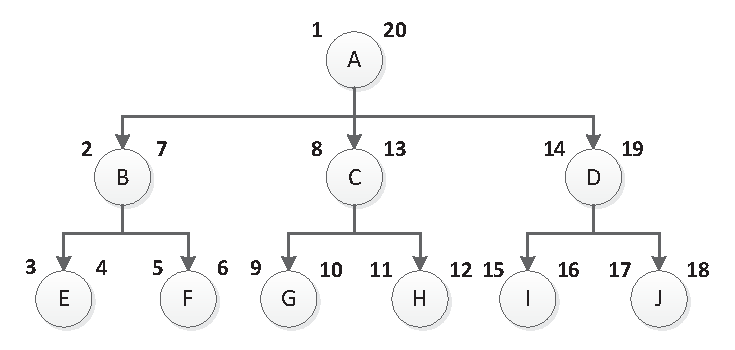
\includegraphics[width=3.3in]{images/tree-lr.eps}
\caption{Example of a tree in nested set model.\label{fig:tree-lr}}
\end{center}
\end{figure}

The left and right (LR) values puts an order on the nodes in the database and establish the following property.

\begin{property}\label{p_ns_desc}
Given two nodes $a$ and $d$, $d$ is a descendant of $a$ if $(a.L < d.L)$ and $(a.R > d.R)$.
\end{property}


\subsection{Operations}

In this section we present how the operations defined can be implemented in the nested sets model. Due to the fact that the nested sets model is an extension of the adjacency list model, implementation of all operations still work in this model; however, the performance (in terms of time of query) of some operations can be improved taking advantage of the left and right values provided by this model.

The simple operations in the previous model cannot be improved further. These operations are Root, Parent, Children and Siblings. We use the same code as provided earlier.

%The Height operations, unfortunately, also cannot be improved much further. The reason is that although the nest model provides a hierarchical information such that a node is member of another node, it does not

Other operations we can improve efficiency using this model. In previous section, we use iterations (loops or recursions) to realize some of the operations, where in each iteration, one query is submitted to the database. Using nested sets model, in most cases however, we can reduce iterations used in the adjacency model to a single query. The operations we can improve include Leaves, Height, Depth, Path, Member, and Tree.

\subsubsection{Leaves Operation}

The Leaves operation no longer require traversal to the bottom of the tree and more importantly required to visit every node in the tree. With the structural information provided by the LR values, we can find the leaf nodes by looking for nodes with the correct LR boundaries that do not have child node. Listing~\ref{ns_leaves} shows the query to accomplish, given an sample input node of $\{ID:B, L:2, R:7\}$.

\begin{lstlisting}[language=sql,caption={Nested Sets Leaves Operation},label=ns_leaves, float]
SELECT * from Nodes N WHERE L > 2 AND R < 7 AND NOT EXIST (SELECT * FROM Nodes WHERE Parent=N.ID) 
\end{lstlisting}

The illustrated query is a correlated query\footnote{http://en.wikipedia.org/wiki/Correlated\_subquery}. The outer query (select) simply limits the selected nodes to be the descendants of input node. For each selected node in the outer query, the subquery checks if there is any child node.

The outer query can be accomplished through two index scans, with the time-complexity of $O(2\log |N|)$. The inner query is the same as the children operation discussed in section~\ref{sec_al_trivial_ops}, which in worst case is also $O(\log |N|)$. With the total complexity of $O(2\log^2 |N|)$, which has a growth rate similar to $O(\log |N|)$.

%This query simply reads find all descendant of node B (L > 2 and R < 7) that does not have any children (nested query).

\subsubsection{Path, Depth, Member Operations}

In addition to the implementation illustrated in Section~\ref{sec_al_depth}, we can also evaluate these operations using the nested sets model, which can be directly obtained from Property~\ref{p_ns_desc}. Path is simply a list of ancestors, which we can easily obtain, and the query node itself. Similarly, Depth is the count of the number of records returned from Path Given an input node of $\{ID:E, L:3, R:4\}$, Listing~\ref{ns_ops} shows the query for Path(line 1-2), and Depth(line 4-5).

\begin{lstlisting}[language=sql,caption={Path, Depth, Member Operations},label=ns_ops, float]
-- Path Query
SELECT * FROM Nodes WHERE L <= 3 AND R >= 4 ORDER BY L

-- Depth Query
SELECT COUNT(*) FROM Nodes WHERE L <= 3 AND R >= 4
\end{lstlisting}

The implementation presented in Section~\ref{sec_al_depth} (using pure adjacency list) and the implementation presented in this section (using LR-values) both have the time complexity of $O(\log |N|)$. For the pure adjacency list implementation, this is easy to see because the number of nodes to search is simply the depth, which is proportional to $log\ |N|$.  As for the implementation in this section, the query evaluator will have to traverse the index tree for the L and R fields to find the qualifying nodes, which also produce $\log$ time-complexity.

Though both produce similar analytical time-complexity, there are differences between the two approaches. The first difference is that the query presented in this section performances the entire evaluation on the database server and sends the final result back to the client; whereas, the logic of the approach of Section~\ref{sec_al_depth} is located on the client, therefore, the server has to send intermediate results back to the client. In other words, the adjacency list implementation requires multiple queries and and results sent between the client and the server. The second difference is that the nested set approach has to traverse the index tree for both R and L fields. The adjacency list approach does not have this complexity.

%\subsubsection{Height}

%Initially it appear that we cannot improve Height using the nested sets model. The left and right values does provide an hierarchical relationship to the data, but how can we use this information to find the longest path from root to a leaf node?

%After some thought, we can use Depth to find the Height of a tree. The Height of a tree is the maximum depth of leaf nodes that are descendants of the root. Listing~\ref{ns_height} shows the query.

%\begin{lstlisting}[language=sql,caption={Height Operation},label=ns_height, float]
%SELECT * from Nodes N WHERE L >= 1 AND R <= 20 AND NOT EXIST (SELECT * FROM Nodes WHERE Parent=N.ID)
%\end{lstlisting}

\subsubsection{Member Operation}

Member match exactly the definition of Property~\ref{p_ns_desc}. Listing~\ref{ns_member} shows a trivial code for this operation.

\begin{lstlisting}[language=java,caption={Member Operation},label=ns_member, float]
static boolean Member(Node n, Node t)
{
    return (t.L < n.L) && (t.R > n.R);
}
\end{lstlisting}

The time complexity of this operation is $O(1)$.

%With nested set model, finding ancestors of a node becomes trivial. Because the left-value of a node is assigned before any child-node is traversed and the right-value after, any \emph{ancestor}, denoted by $a$, of a node $n$ has the following properties:

%\begin{enumerate}
%\item $a.left < n.left$
%\item $n.right < a.right$
%\end{enumerate}

%\textbf{Note:} ``left'' and ``right'' are SQL keywords, consider changing left to another name.\\

%With the above properties, the queries for ancestors no longer require multiple queries (or recursion). Listing~\ref{ns_ancestors} shows the query to get ancestors of node $E$ in Figure~\ref{fig:tree-lr}.

%\begin{lstlisting}[language=sql,caption={Query for ancestors for node $E$ via nested set model},label=ns_ancestors, float]
%SELECT * FROM Nested_Set WHERE Left < 3 AND Right > 4
%\end{lstlisting}

\subsubsection{Tree}

Getting the entire hierarchy of a tree is the same as getting all the descendants of the root node (including the root). If the database contains only one tree, then this operation involves retrieving all entries in the nodes table. However, we assume that the database contains multiple disconnected trees.

Listing~\ref{ns-tree} shows this query for the tree in Figure~\ref{fig:tree-lr}, in which the left and right value for the root node $A$ is 1 and 20, respectively.

\begin{lstlisting}[language=sql,caption={Query for Tree for tree $A$ via nested set model},label=ns-tree, float]
SELECT * FROM Nested_Set WHERE Left > 1 AND Right < 20 ORDER BY left ASC
\end{lstlisting}

To reconstruct the hierarchical structure from the flat list returned from the query above, we look at the result of the query (of the tree in Figure~\ref{ns-tree}) in the Table~\ref{table:ns_tree} below.

\begin{table}[h]
\centering
\begin{tabular}{|l|l|l|l|}
\hline
{\bf ID} & {\bf Left} & {\bf Right} & {\bf Parent} \\ \hline\hline
A & 1 & 20 & null \\ \hline
B & 2 & 7 & A \\ \hline
E & 3 & 4 & B \\ \hline
F & 5 & 6 & B \\ \hline
C & 8 & 13 & A \\ \hline
G & 9 & 10 & C \\ \hline
H & 11 & 12	& C \\ \hline
D & 14 & 19	& A \\ \hline
I & 15 & 16	& D \\ \hline
J & 17 & 18	& D \\ \hline
\end{tabular}
\caption{Query result of Tree operation\label{table:ns_tree}}
\end{table}

There are two ways to reconstruct the tree, since there are redundant information in the result table to reconstruct the tree. The first way is to only use the `Parent' column. The second way is to use only the `Left' and `Right' columns (not needing the `Parent' column). Listing~\ref{ns_tree_const1} shows the algorithm for the first approach.

\begin{lstlisting}[language=java,caption={Tree reconstruction using Parent},label=ns_tree_const1, float]
Node ReconstructTree(List<Record> records)
{
    Node root, current = null;
    for(Record record : records)
    {
        if(current == null)
        {
            current = MakeNode(record);
            root = current;
        }
        else
        {
            while(current.ID != record["Parent"])
                current = current.Parent;

            Node node = MakeNode(record);
            current.Children.Add(node);
            current = node;
        }
    }
	return root;
}
\end{lstlisting}

Listing~\ref{ns_tree_const2} shows the algorithm for the second approach.

\begin{lstlisting}[language=java,caption={Tree reconstruction using Left and Right value},label=ns_tree_const2, float]
//Returns the root node as the tree
Node ReconstructTree(List<Record> records)
{
    Node root, current = null;
    for(Record record : records)
    {
        if(current == null) //This should only be run once
        {
            current = MakeNode(record);
            root = current;
        }        
        else
		{
            while(!(current.Left < record["Left"] and current.Right > record["Right"]))
                current = current.Parent;
                
            Node node = MakeNode(record);
            current.Children.Add(node);
            current = node;
        }
    }
    return root;
}
\end{lstlisting}	

\subsubsection{Print Tree}

The tree structure can be easily outputted by a program after the hierarchy has been reconstructed with the algorithms in the previous section. However, sometimes a tree has large number of nodes and we may only need to output the tree structure without needing to reconstruct the tree in memory.

This section shows an algorithm to print the ID of the nodes with increasing indention to show the hierarchy of the tree.

\begin{lstlisting}[caption={Tree reconstruction using Left and Right value},label=ns_print_tree, float]
void PrintTree(List<Record> records)
	//Make new stack to hold right values; 
	//length = 0
	Stack stack;
	foreach(Record record in records)
		while(stack.top < record["right"] and !stack.isEmpty)
			stack.pop()
		//Print indentation
		for(int i = 0 to stack.length - 1) 
			Print(" ")
		//Print current record
		Print(Record.ID)
		stack.push(record["right"])
\end{lstlisting}

\section{Evaluation}

This section presents the performance evaluation of the adjacency list and nested sets models presented in section~\ref{sec-adj-list} and \ref{sec-nested-set}, respectively. Performance are evaluated based on the running time of the operations described in section~\ref{sec_tree_ops}, under each data model.

The evaluation is composed of two parts: the server and the client. The server runs an instance of MySQL database and holds hierarchical structure and data. The client connects to the server via local area network, implements the operations, and reports the amount of time to run them.

This section is organized as follows. Section~\ref{sec-server-config} and section~\ref{sec-client-config} describe the environment and configuration of the server and the client.

\subsection{Server Configuration}\label{sec-server-config}

Table~\ref{table:tbl_server_config} shows the software and hardware configuration of the server machine.

\begin{table}[h]
\centering
\begin{tabular}{|l|l|}
\hline
CPU & Intel Processor 64-bit \\ \hline
Memory & 4 GB \\ \hline
Operating System & Ubuntu 13.10 \\ \hline
Database System & MySQL 5.5 Community Edition \\ \hline 
\end{tabular}
\caption{Dataset size\label{table:tbl_server_config}}
\end{table}

In addition, when running the database system, the following settings are made:

\begin{table}[h]
\centering
\begin{tabular}{|l|l|l|}
\hline
Variable & Set Value & Default Value \\ \hline
max\_sp\_recursion\_depth & 100 & 0 \\ \hline
maximum\_stack memory & 100 & 100 \\ \hline
some other memory & 100 & 100 \\ \hline
\end{tabular}
\caption{Database Server Non-default Settings\label{table:tbl_server_settings}}
\end{table}

Note: briefly describe the reason for above settings.

\subsection{Client Configuration}\label{sec-client-config}

The client machine is responsible for running the experiment code, which is written in Java and connected to the database using MySQL JDBD Connector\footnote{http://www.oracle.com/technetwork/java/javase/jdbc/index.html}. Table~\ref{tbl-client-config} lists configurations of the client environment.

\begin{table}[h]
\centering
\begin{tabular}{|l|l|}
\hline
CPU & Intel Processor 64-bit \\ \hline
Memory & 12 GB \\ \hline
Operating System & Ubuntu 13.10 Desktop \\ \hline
Programming Language & Java 7 (OpenJDK 7) \\ \hline
Database Connector   & JDBC mysql-connector-java-5.1.29 \\ \hline
\end{tabular}
\caption{Dataset size\label{tbl-client-config}}
\end{table}

At early stages of coding the experiments, the author repeatedly getting Out Of Memory Error from the Java Virtual Machine. The code for the experiments have been rewritten several times to reduce memory consumption. The error can also be mitigated by expanding the allocated memory to the program. The following are the command sets the minimum and maximum heap memory allocated to the experiment to 8 and 9 gigabytes.

\begin{lstlisting}[language=bash,caption={Nodes table for nested set model},label=run_client, float]
java -cp lib/mysql-connector-java-5.1.29-bin.jar:. -Xms8g -Xmx9g Experiment
\end{lstlisting}

\subsection{Data Format and Generation}\label{sec_experimental_data}

The experimental datasets are synthetically generated relational hierarchies, each containing the fields ID, Parent, L and R as described for the Nodes table in Listing~\ref{ns_schema}. In addition, each record (an entry in data table) also contains additional 90 ASCII characters, divided into two fields (45 characters each), to simulate data payload in typical database record. However, these additional data is currently not being used in experiments, due to the limitation of amount of memory in machines that run the experiments. The structure of the experimental data shown in Table~\ref{tb_rel_exp_data_format}.

\begin{table}[h]
\centering
\begin{tabular}{|l|l|l|l|l|l|}
\hline
\textbf{Field} & \textbf{Type} & \textbf{Null} & \textbf{Key} & \textbf{Default} & \textbf{Extra}  \\ \hline
id             & int(11)       & NO            & PRI          & NULL             & auto\_increment \\ \hline
parent         & int(11)       & YES           & MUL          & NULL             &                 \\ \hline
l              & int(11)       & NO            & MUL          & NULL             &                 \\ \hline
r              & int(11)       & NO            & MUL          & NULL             &                 \\ \hline
data1          & varchar(45)   & NO            &              & NULL             &                 \\ \hline
data2          & varchar(45)   & NO            &              & NULL             &                 \\ \hline
\end{tabular}
\caption{Experimental data relational format}
\label{tb_rel_exp_data_format}
\end{table}

The datasets are created by our data generation SQL script (see appendix) and stored on in the database on the server. In addition to being a full tree\footnote{http://en.wikipedia.org/wiki/Binary\_tree\#Types\_of\_binary\_trees}, each dataset is characterized by the following properties:

\begin{enumerate}
\item Order: the number of children per node. This is also known as the fan-out or out-degree of a tree.
\item Height: the number of nodes of the longest path from root to a leaf node.
\end{enumerate} 

Each of the properties ranges from 2 to 10, with the exception that higher-order datasets have lower max height. For each combination of order and height, a dataset is generated and stored in a database table. Table~\ref{tbl:reltree_data_size} shows the size (number of records) of each data table.

\newcommand*\rot{\rotatebox{90}}

\begin{table}[h]
\centering
\begin{tabular}{lc|r|r|r|r|r|r|r|r|r|}
\cline{3-11}
 & \multicolumn{1}{l}{} & \multicolumn{9}{|c|}{\textbf{Height}} \\ \cline{3-11} 
 & \multicolumn{1}{l}{} & \multicolumn{1}{|c}{\textbf{2}} & \multicolumn{1}{|c}{\textbf{3}} & \multicolumn{1}{|c}{\textbf{4}} & \multicolumn{1}{|c}{\textbf{5}} & \multicolumn{1}{|c}{\textbf{6}} & \multicolumn{1}{|c}{\textbf{7}} & \multicolumn{1}{|c}{\textbf{8}} & \multicolumn{1}{|c}{\textbf{9}} & \multicolumn{1}{|c|}{\textbf{10}} \\ \hline
\multicolumn{1}{|l}{\multirow{9}{*}{\rot{\textbf{Order}}}} & \multicolumn{1}{|c|}{\textbf{2}} & 3 & 7 & 15 & 31 & 63 & 127 & 255 & 511 & 1,023 \\ \cline{2-11} 
\multicolumn{1}{|l}{\textbf{}} & \multicolumn{1}{|c|}{\textbf{3}} & 4 & 13 & 40 & 121 & 364 & 1,093 & 3,280 & 9,841 & 29,524 \\ \cline{2-11} 
\multicolumn{1}{|l}{\textbf{}} & \multicolumn{1}{|c|}{\textbf{4}} & 5 & 21 & 85 & 341 & 1,365 & 5,461 & 21,845 & 87,381 & 349,525 \\ \cline{2-11} 
\multicolumn{1}{|l}{\textbf{}} & \multicolumn{1}{|c|}{\textbf{5}} & 6 & 31 & 156 & 781 & 3,906 & 19,531 & 97,656 & 488,281 & 2,441,406 \\ \cline{2-11} 
\multicolumn{1}{|l}{\textbf{}} & \multicolumn{1}{|c|}{\textbf{6}} & 7 & 43 & 259 & 1,555 & 9,331 & 55,987 & 335,923 & 2,015,539 & 12,093,235 \\ \cline{2-11} 
\multicolumn{1}{|l}{\textbf{}} & \multicolumn{1}{|c|}{\textbf{7}} & 8 & 57 & 400 & 2,801 & 19,608 & 137,257 & 960,800 & 6,725,601 & 47,079,208 \\ \cline{2-11} 
\multicolumn{1}{|l}{\textbf{}} & \multicolumn{1}{|c|}{\textbf{8}} & 9 & 73 & 585 & 4,681 & 37,449 & 299,593 & 2,396,745 & 19,173,961 & 153,391,689 \\ \cline{2-11} 
\multicolumn{1}{|l}{\textbf{}} & \multicolumn{1}{|c|}{\textbf{9}} & 10 & 91 & 820 & 7,381 & 66,430 & 597,871 & 5,380,840 & 48,427,561 & 435,848,050 \\ \cline{2-11} 
\multicolumn{1}{|l}{\textbf{}} & \multicolumn{1}{|c|}{\textbf{10}} & 11 & 111 & 1,111 & 11,111 & 111,111 & 1,111,111 & 11,111,111 & 111,111,111 & 1,111,111,111 \\ \hline
\end{tabular}
\caption{Test data size with respect to Order and Height}
\label{tbl:reltree_data_size}
\end{table}

With the server configuration described earlier in this section, an estimate of the amount of time to generate the data sets is shown in Table~\ref{tb_rel_data_gentime_est}.

% Please add the following required packages to your document preamble:
% \usepackage{multirow}
\begin{table}[h]
\centering
\begin{tabular}{cc|c|c|c|c|c|c|c|c|c|}
\cline{3-11}
                                                     &                                   & \multicolumn{9}{|c|}{\textbf{Height}}                                                                               \\ \cline{3-11} 
                                                     &                                   & \textbf{2} & \textbf{3} & \textbf{4} & \textbf{5} & \textbf{6} & \textbf{7} & \textbf{8} & \textbf{9} & \textbf{10} \\ \hline
\multicolumn{1}{|c}{\multirow{9}{*}{\rot{\textbf{Order}}}} & \multicolumn{1}{|c|}{\textbf{2}}  & 200 ms     & 470 ms     & 470 ms     & 2.07 sec   & 4.2 sec    & 8.47 sec   & 17 sec     & 34.07 sec  & 1.14 min    \\ \cline{2-11} 
\multicolumn{1}{|c}{\textbf{}}                       & \multicolumn{1}{|c|}{\textbf{3}}  & 270 ms     & 870 ms     & 2.67 sec   & 8.07 sec   & 24.27 sec  & 1.21 min   & 3.64 min   & 10.93 min  & 32.80 min   \\ \cline{2-11} 
\multicolumn{1}{|c}{\textbf{}}                       & \multicolumn{1}{|c|}{\textbf{4}}  & 330 ms     & 1.4 sec    & 5.67 sec   & 22.73 sec  & 1.52 min   & 6.07 min   & 24.27 min  & 1.62 hr    & 6.47 hr     \\ \cline{2-11} 
\multicolumn{1}{|c}{\textbf{}}                       & \multicolumn{1}{|c|}{\textbf{5}}  & 400 ms     & 2.07 sec   & 10.4 sec   & 52.07 sec  & 4.34 min   & 21.7 min   & 1.81 hr    & 9.04 hr    & 1.88 days   \\ \cline{2-11} 
\multicolumn{1}{|c}{\textbf{}}                       & \multicolumn{1}{|c|}{\textbf{6}}  & 470 ms     & 2.86 sec   & 17.27 sec  & 1.73 min   & 10.37 min  & 1.04 hr    & 6.22 hr    & 1.56 days  & 9.33 days   \\ \cline{2-11} 
\multicolumn{1}{|c}{\textbf{}}                       & \multicolumn{1}{|c|}{\textbf{7}}  & 530 ms     & 3.8 sec    & 26.67 sec  & 3.11 min   & 21.79 min  & 2.54 hr    & 17.79 hr   & 5.19 days  & 36.33 days  \\ \cline{2-11} 
\multicolumn{1}{|c}{\textbf{}}                       & \multicolumn{1}{|c|}{\textbf{8}}  & 600 ms     & 4.87 sec   & 39 sec     & 5.20 min   & 41.61 min  & 5.55 hr    & 1.85 days  & 14.79 days & 118.36 days \\ \cline{2-11} 
\multicolumn{1}{|c}{\textbf{}}                       & \multicolumn{1}{|c|}{\textbf{9}}  & 670 ms     & 6.07 sec   & 54.67 sec  & 8.20 min   & 1.23 hr    & 11.07 hr   & 4.15 days  & 37.37 days & 336.30 days \\ \cline{2-11} 
\multicolumn{1}{|c}{\textbf{}}                       & \multicolumn{1}{|c|}{\textbf{10}} & 730 ms     & 7.4 sec    & 1.23 min   & 12.35 min  & 2.06 hr    & 20.58 hr   & 8.57 days  & 85.73 days & 857.34 days \\ \hline
\end{tabular}
\caption{Experimental data generation time estimate}
\label{tb_rel_data_gentime_est}
\end{table}


\subsection{Experimental Result}\label{sec_rt_eval_result}

The operations defined in Section~\ref{sec_tree_ops} are divided into three categories based on their running time complexity which are $O(log N)$, $O(N)$, and $O(1)$. Members in a category have the similar running time; therefore we have to show the performance for one operation per group. The membership of each category shows as follows:

\begin{enumerate}
\item $O(log N)$ : Root, Depth, Path, Member
\item $O(N)$ : Heaves, Height, Tree
\item $O(1)$ : Parent, Children, Siblings
\end{enumerate}

In this section, we report the performance of category 1 and 2. Category 3 is not reported since the input size does not affect the outcome and that the implementation are the same for both adjacency-list and nested-sets model.

\subsubsection{Category 1 - O(log N)}\label{eval_group1}

Figure~\ref{fig-root-al} depicts the running time in milliseconds of the finding root operation for the adjacency list model. From this result, we can rough infer that the time complexity of this algorithm is linear with respect to the depth, and constant with respect to the width (order) of the tree.

\begin{figure}[!h]
\begin{center}
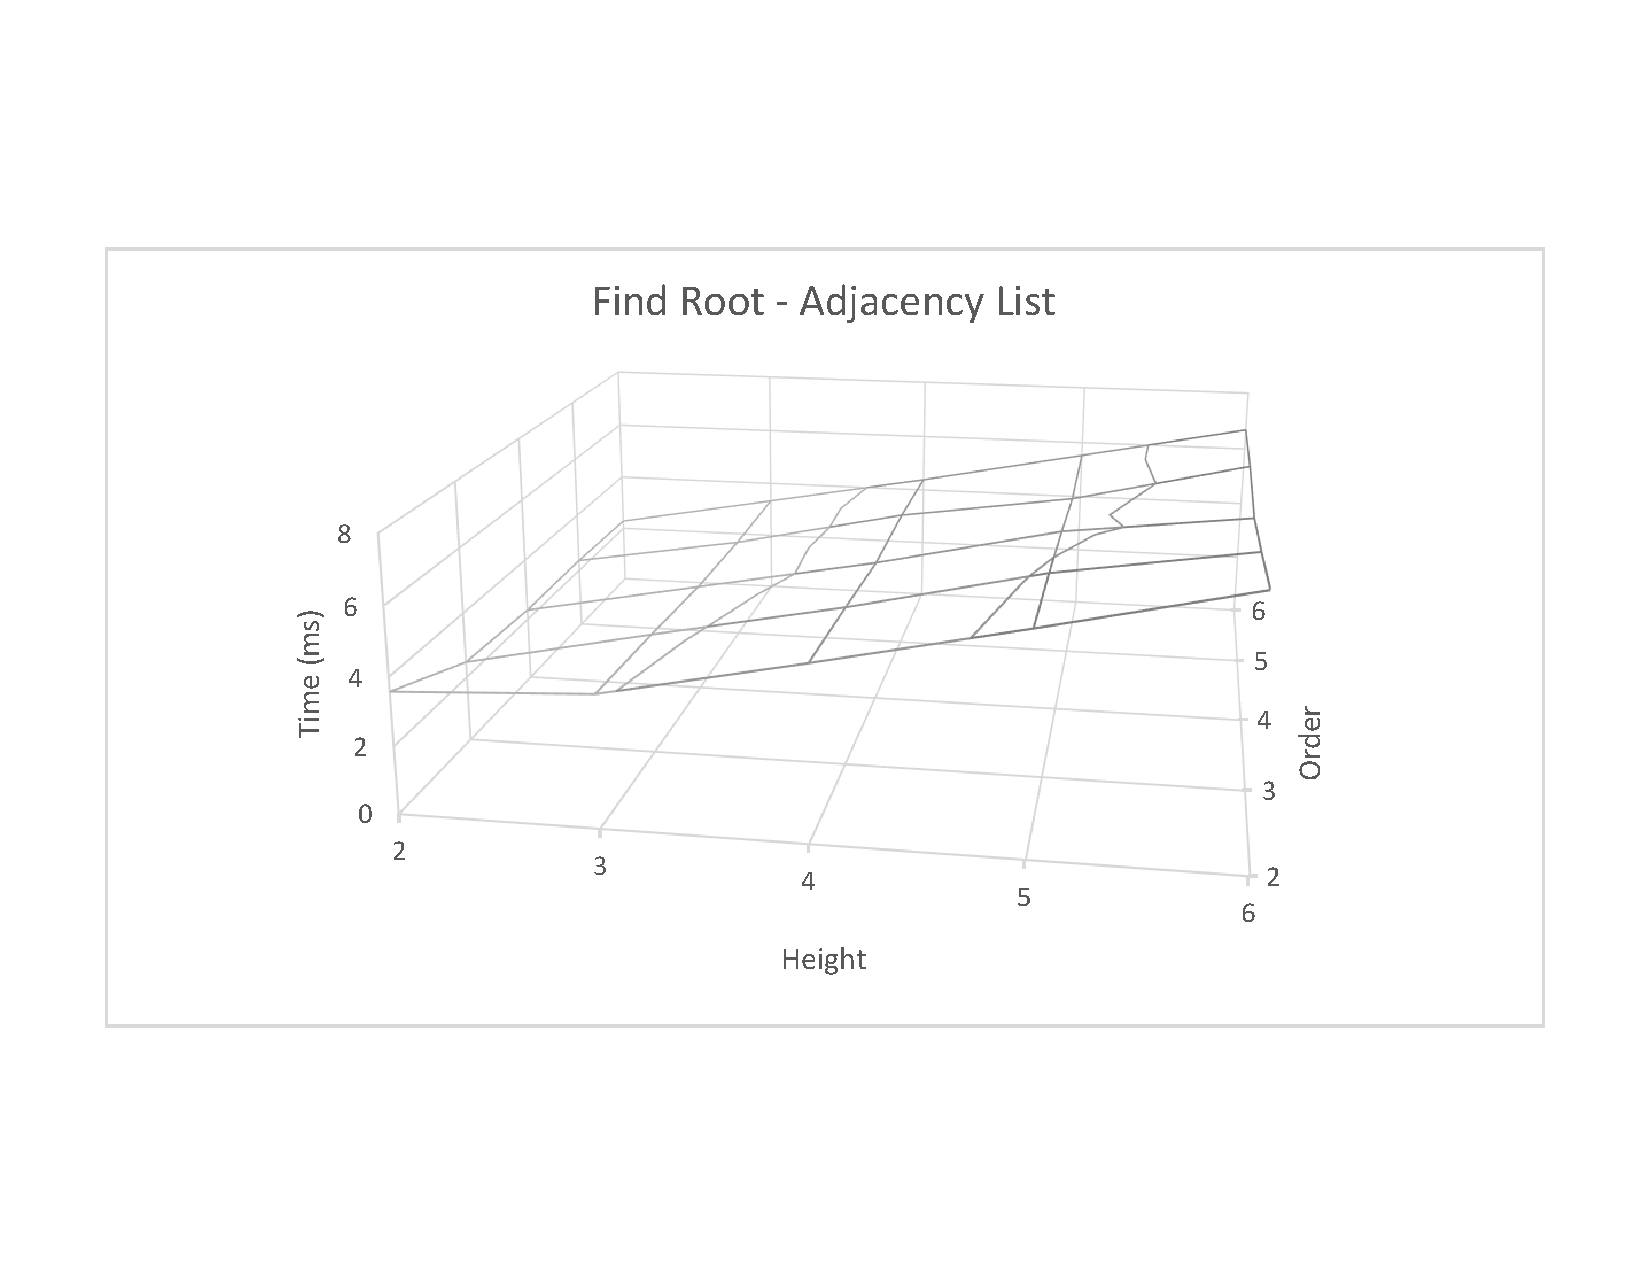
\includegraphics[width=6in]{images/root-al-wire.pdf}
\caption{Running time using Adjacency List Model.\label{fig-root-al}}
\end{center}
\end{figure}

Figure~\ref{fig-root-ns} depicts the running time in milliseconds of the finding root operation for the nested sets model. One can easily see that it is an improvement over the adjacency list model. In this result, the time complexity with increasing depth of the tree has reduced to constant. The time complexity with increasing width stayed constant, with slight constant improvement.

\begin{figure}[!h]
\begin{center}
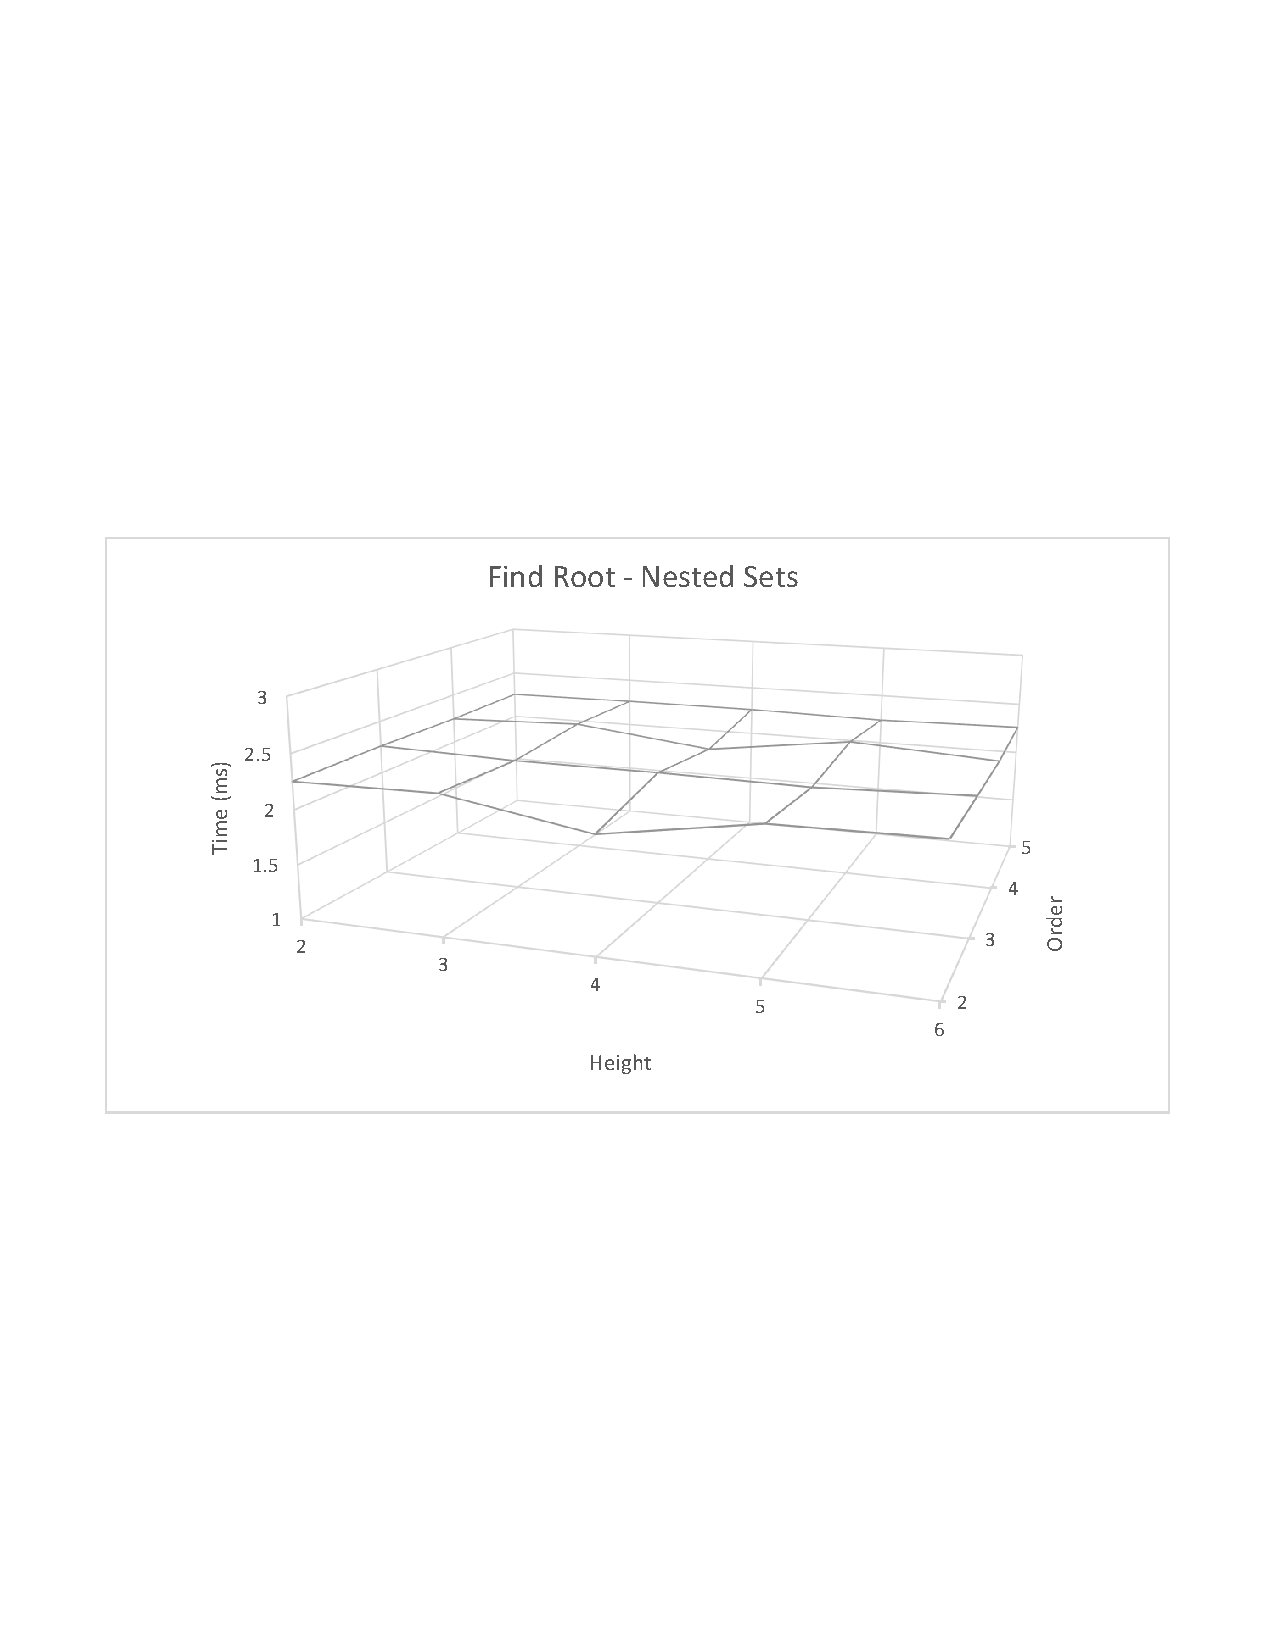
\includegraphics[width=6in]{images/root-ns-wire.pdf}
\caption{Running time using Nested Sets Model.\label{fig-root-ns}}
\end{center}
\end{figure}

If we take a slice of the previous two figures down where height = 8, we can see the growth of the algorithm with respect to order as shown in Figure~\ref{fig-time-order}. The figures shows, as expected, that the growth of the order of the tree has little effect on the running time of the operation.

\begin{figure}[!h]
\begin{center}
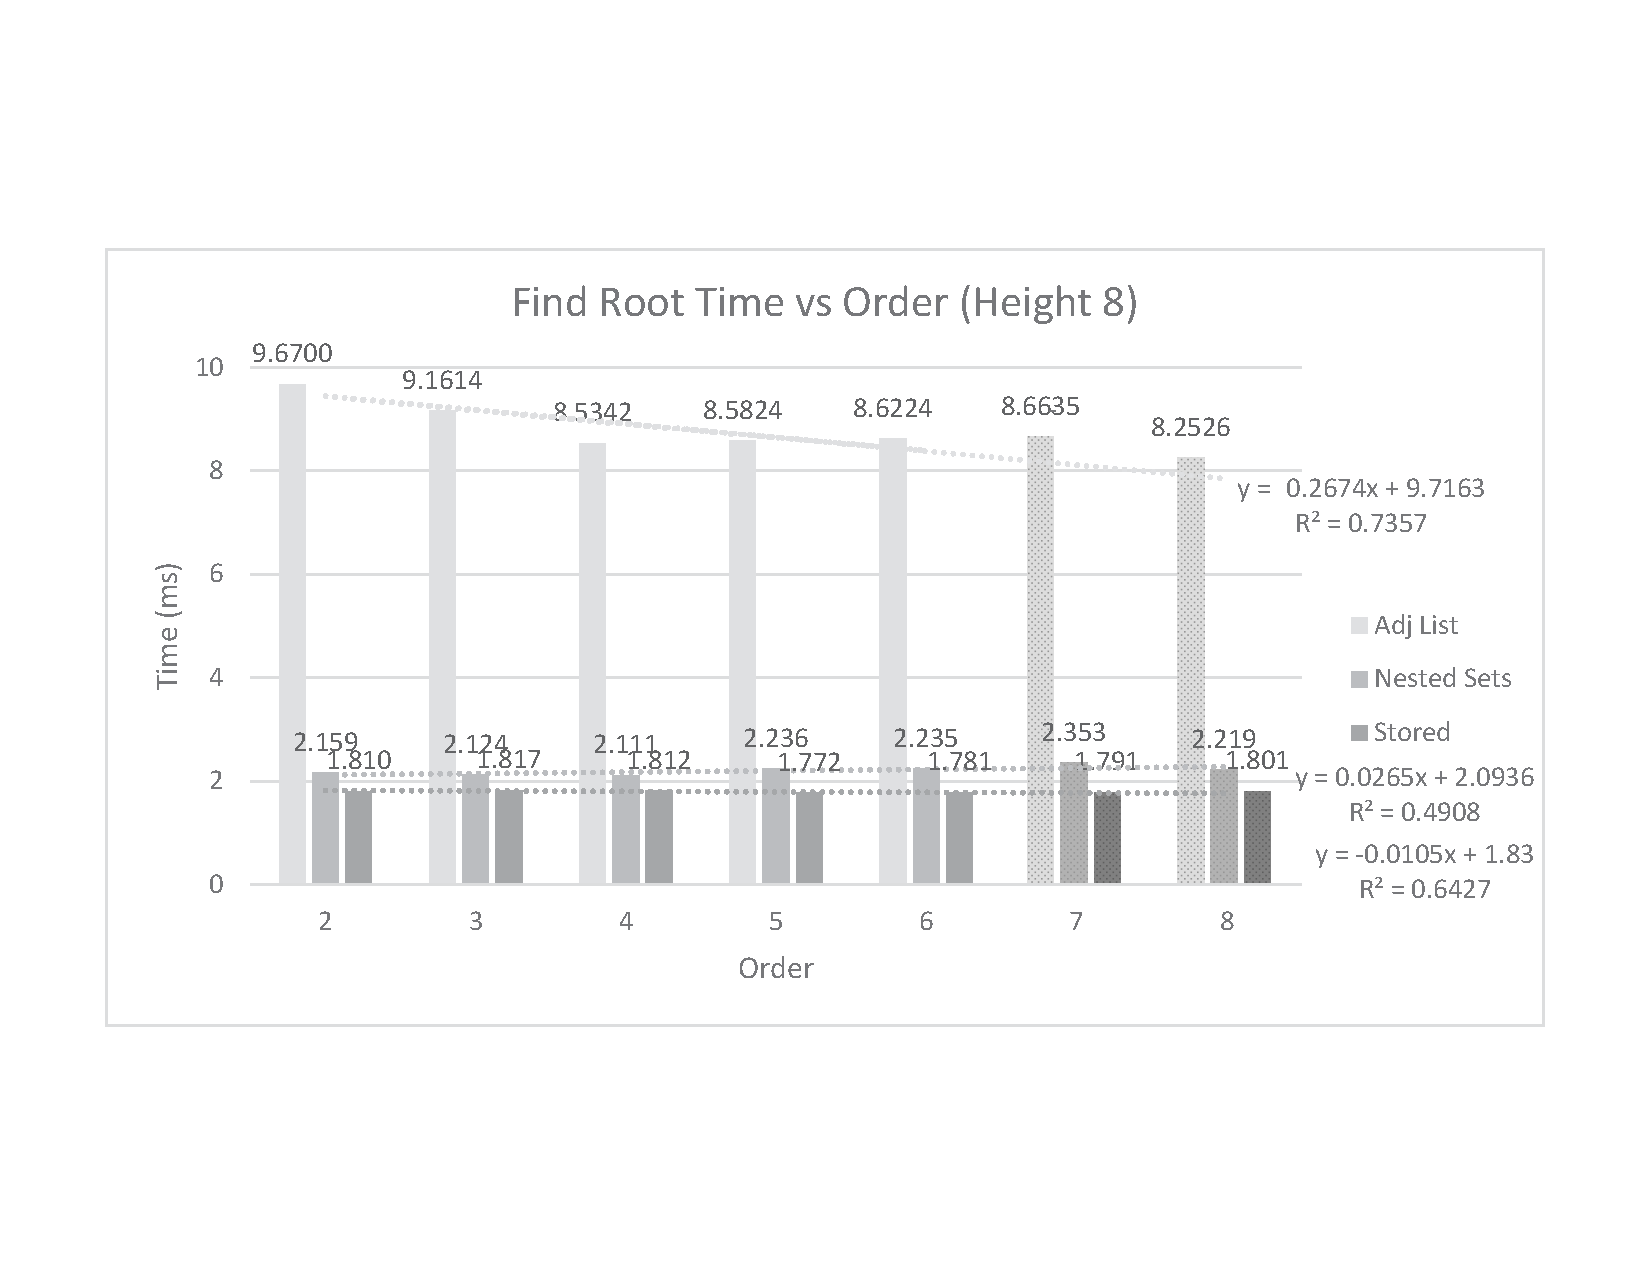
\includegraphics[width=6in]{images/order.pdf}
\caption{Running time vs node out-degree (order) at height = 8.\label{fig-time-order}}
\end{center}
\end{figure}

For the adjacency list model, the trend appears to be decreasing. However if we look at the running time from order 4 to 8, the trend is flat. I believe that the initial decreasing trend is caused by database warm-up. As more data are cached, the database system is able to reach stable-state.

In addition to the two described models, the figure shows the growth trend for adjacency list model implemented using MySQL stored procedure (labeled Stored). The purpose of the stored implementation is to see if stored procedures facilitates performance. In this case, the store version is better than both adjacency list and nested sets models.

In the figure, the trend line is draw using linear regression from the data from order 1 to 6. The measurement of order 7 and 8 are draw to verify the correctness of the growth model.

In the same manner, if we take a slice of Figure~\ref{fig-root-al} and \ref{fig-root-ns} down where order = 8, we can see the growth of the algorithm with respect to height as shown in Figure~\ref{fig-time-height}.

\begin{figure}[!h]
\begin{center}
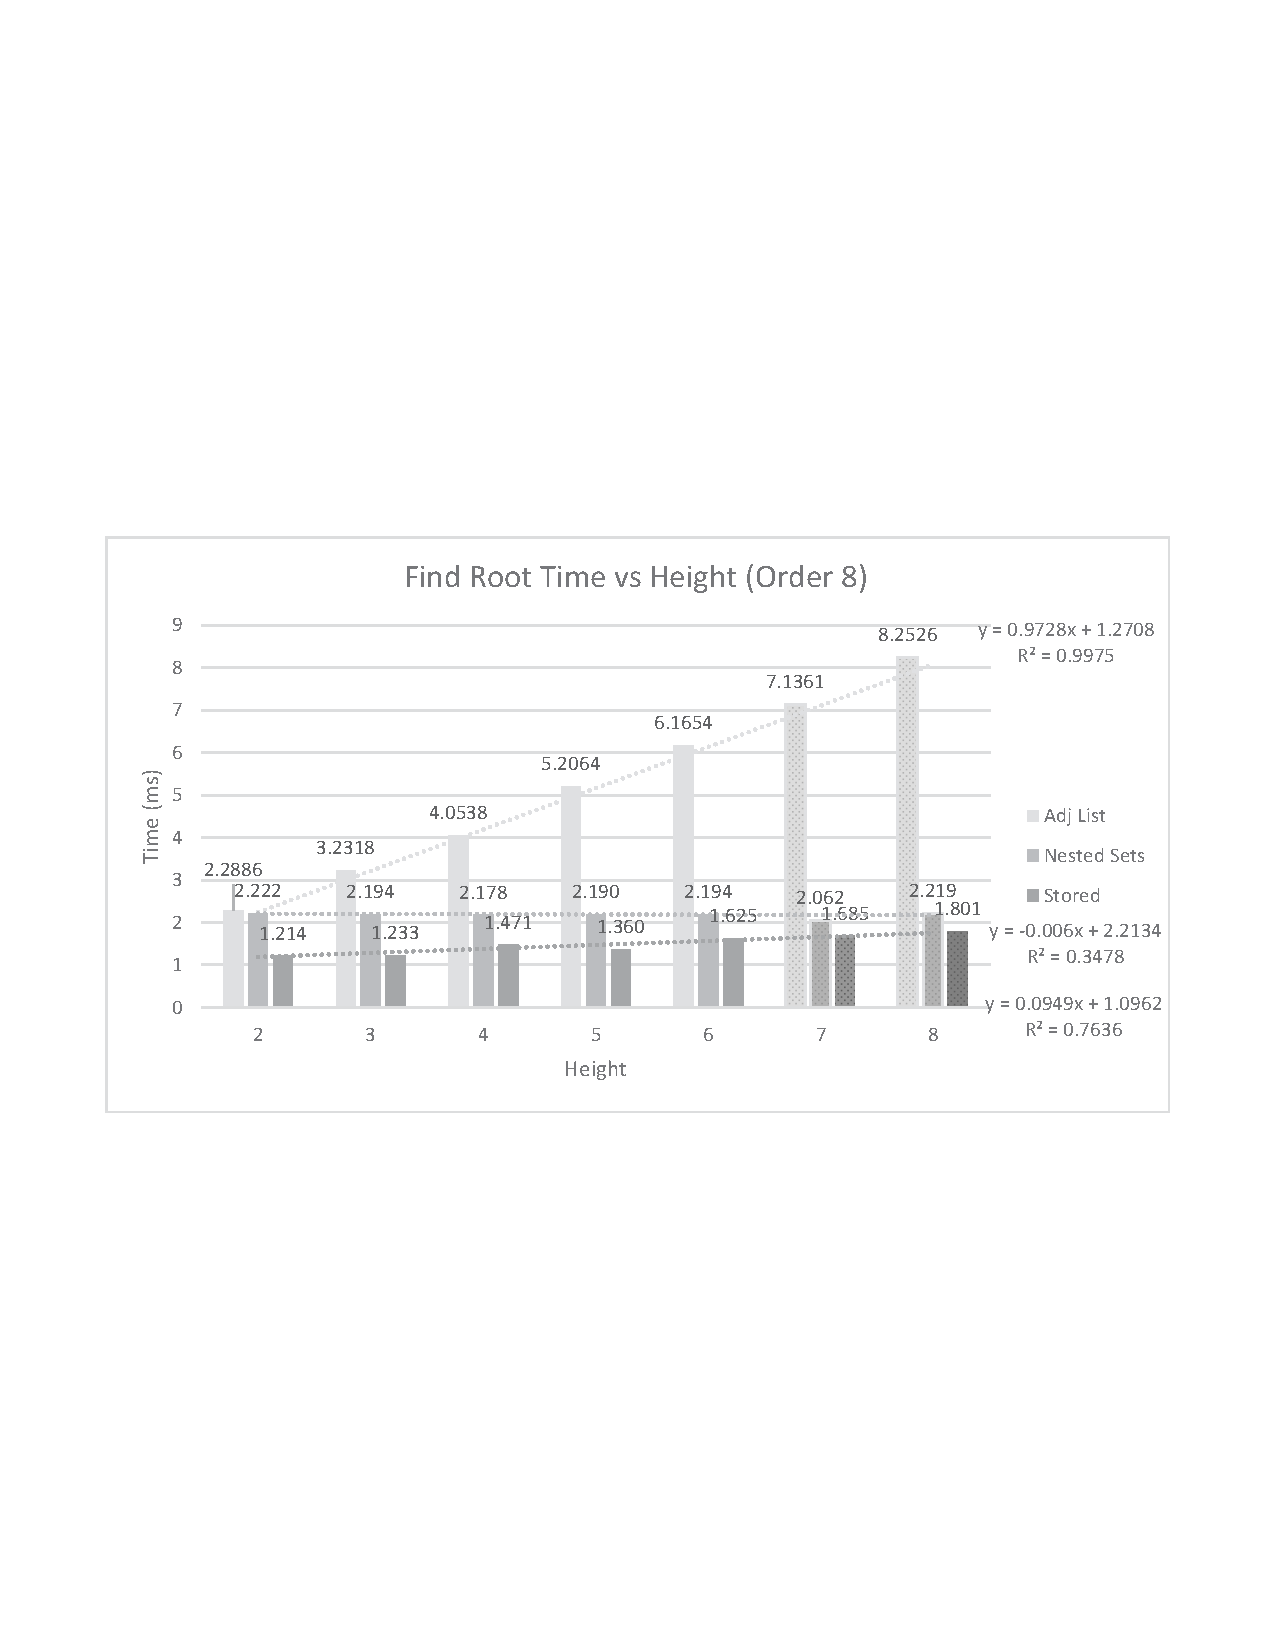
\includegraphics[width=6in]{images/height.pdf}
\caption{Running time vs tree height at order = 8.\label{fig-time-height}}
\end{center}
\end{figure}

The figure shows that for adjacency list model, the running time grows linearly with respect to height. In contract, the running time for the nested sets model shows big improvement over adjacency list, with almost perfect flat trend line model, and indicates constant time-complexity. Once again, the data for the stored model shows that the running time are better than both other models; however, the trend shows a linear growth rate, which is not not better than nested sets model larger data set.


\subsubsection{Category 2 - O(N)}\label{eval_group2}

Figure~\ref{fig-leaves-al} depicts the running time, in milliseconds, of the finding root operation using the Adjacency List Model. The running time stayed relative flat, below 100 ms for height and order, below 4.

Above 4, the figure shows that the running time appears to be growing exponentially with respect to both dimensions. The exponential growth with respect to height is expected because the operation has $O(N)$ complexity and each increase of height increase $N$ by a factor of $w$, where $N$ is the number of nodes and $w$ is the order (or width) of the hierarchy.

However, the exponential growth with respect to the order $w$ in the figure is not expected. Increase in the width of the hierarchy only linearly increase the number of node $N$. This is likely caused by additional processing (such as index tree traversal) required by the database system that makes the cost of all nodes higher than $O(N)$.

\begin{figure}[!h]
\begin{center}
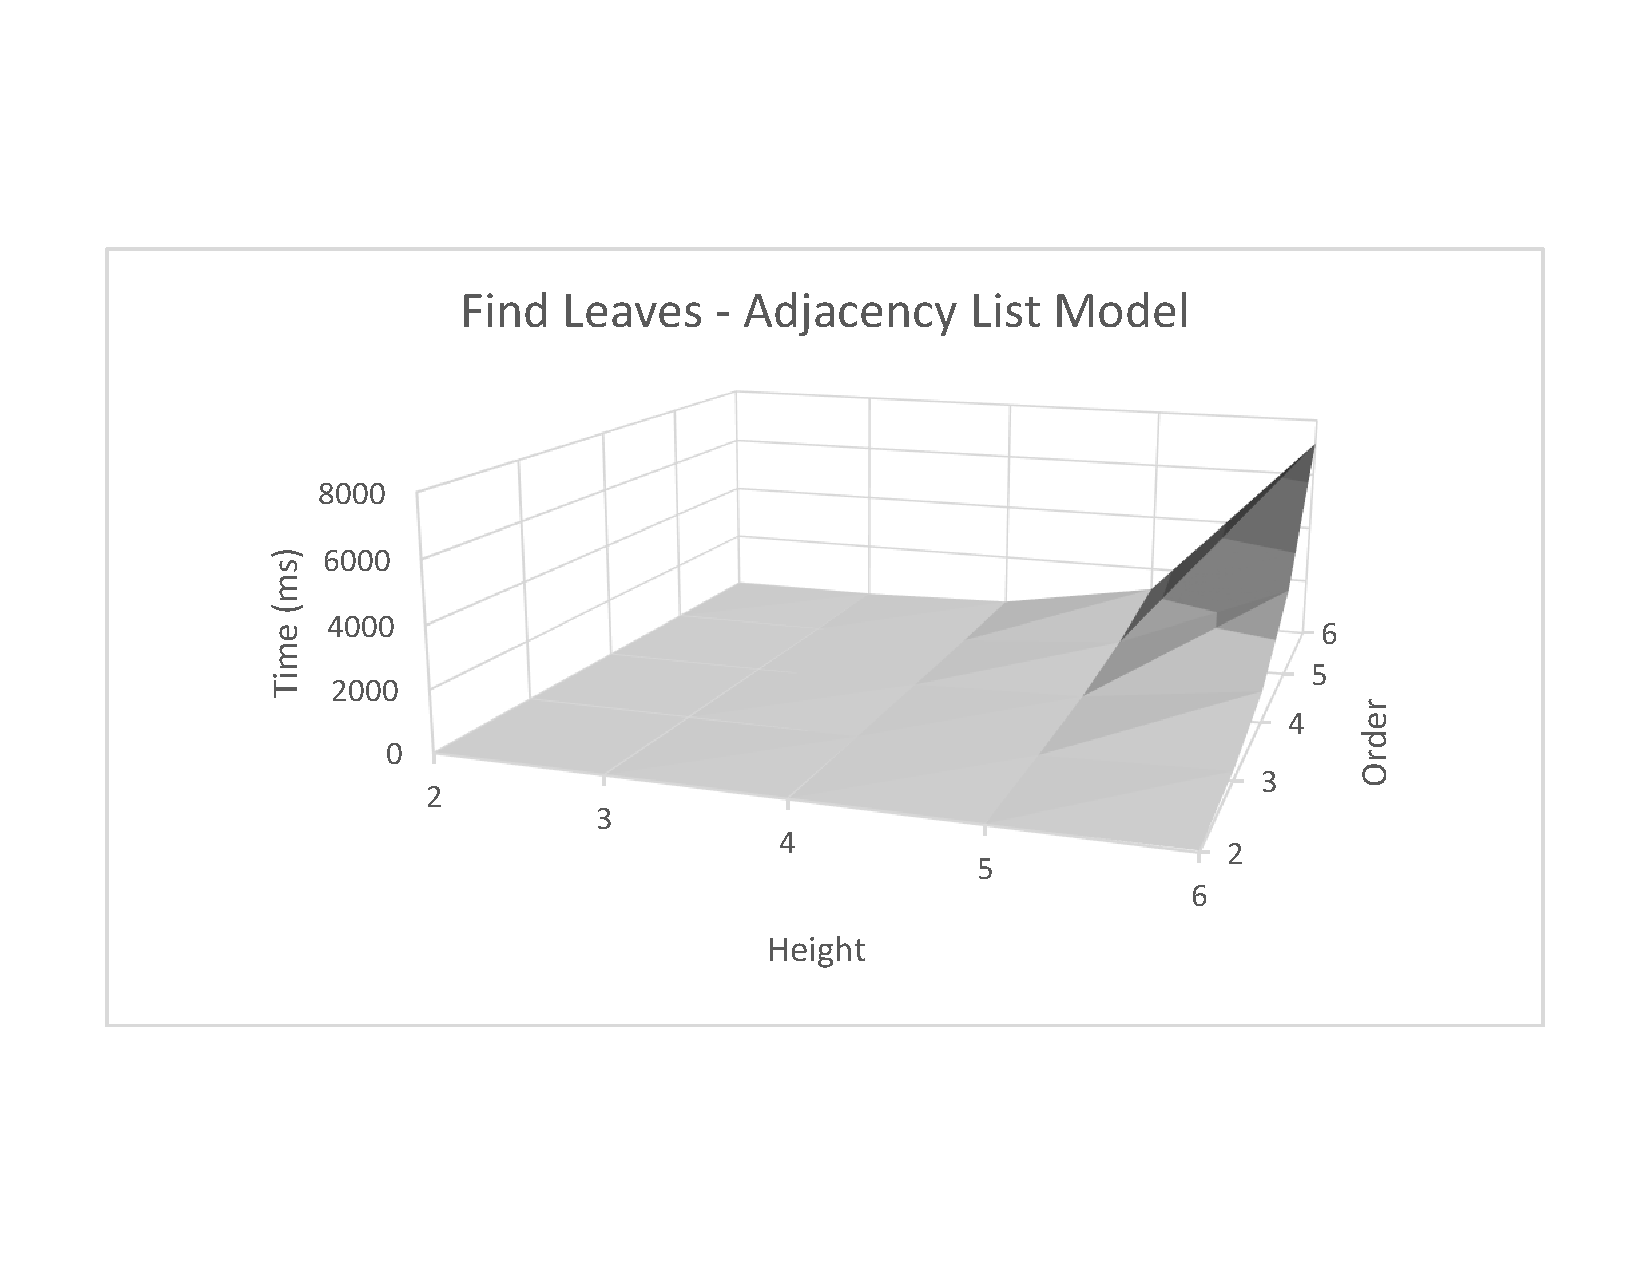
\includegraphics[width=6in]{images/eval/leaves/al_surface.pdf}
\caption{Running time of Finding Leaves using Adjacency List Model.\label{fig-leaves-al}}
\end{center}
\end{figure}


Figure~\ref{fig-leaves-ns} depicts the running time, in milliseconds, of the operation using Nested Sets Model. Careful reader will find that the figure looks almost the same as Figure~\ref{fig-leaves-al}. Although the two figures have the same shape, the running time for the Nested Sets Model is much lower. Taking height = 6 and order = 6 for example, the running time Adjacency List Model is around 7,000 ms, but Nested Sets Model around  9 ms.

\begin{figure}[!h]
\begin{center}
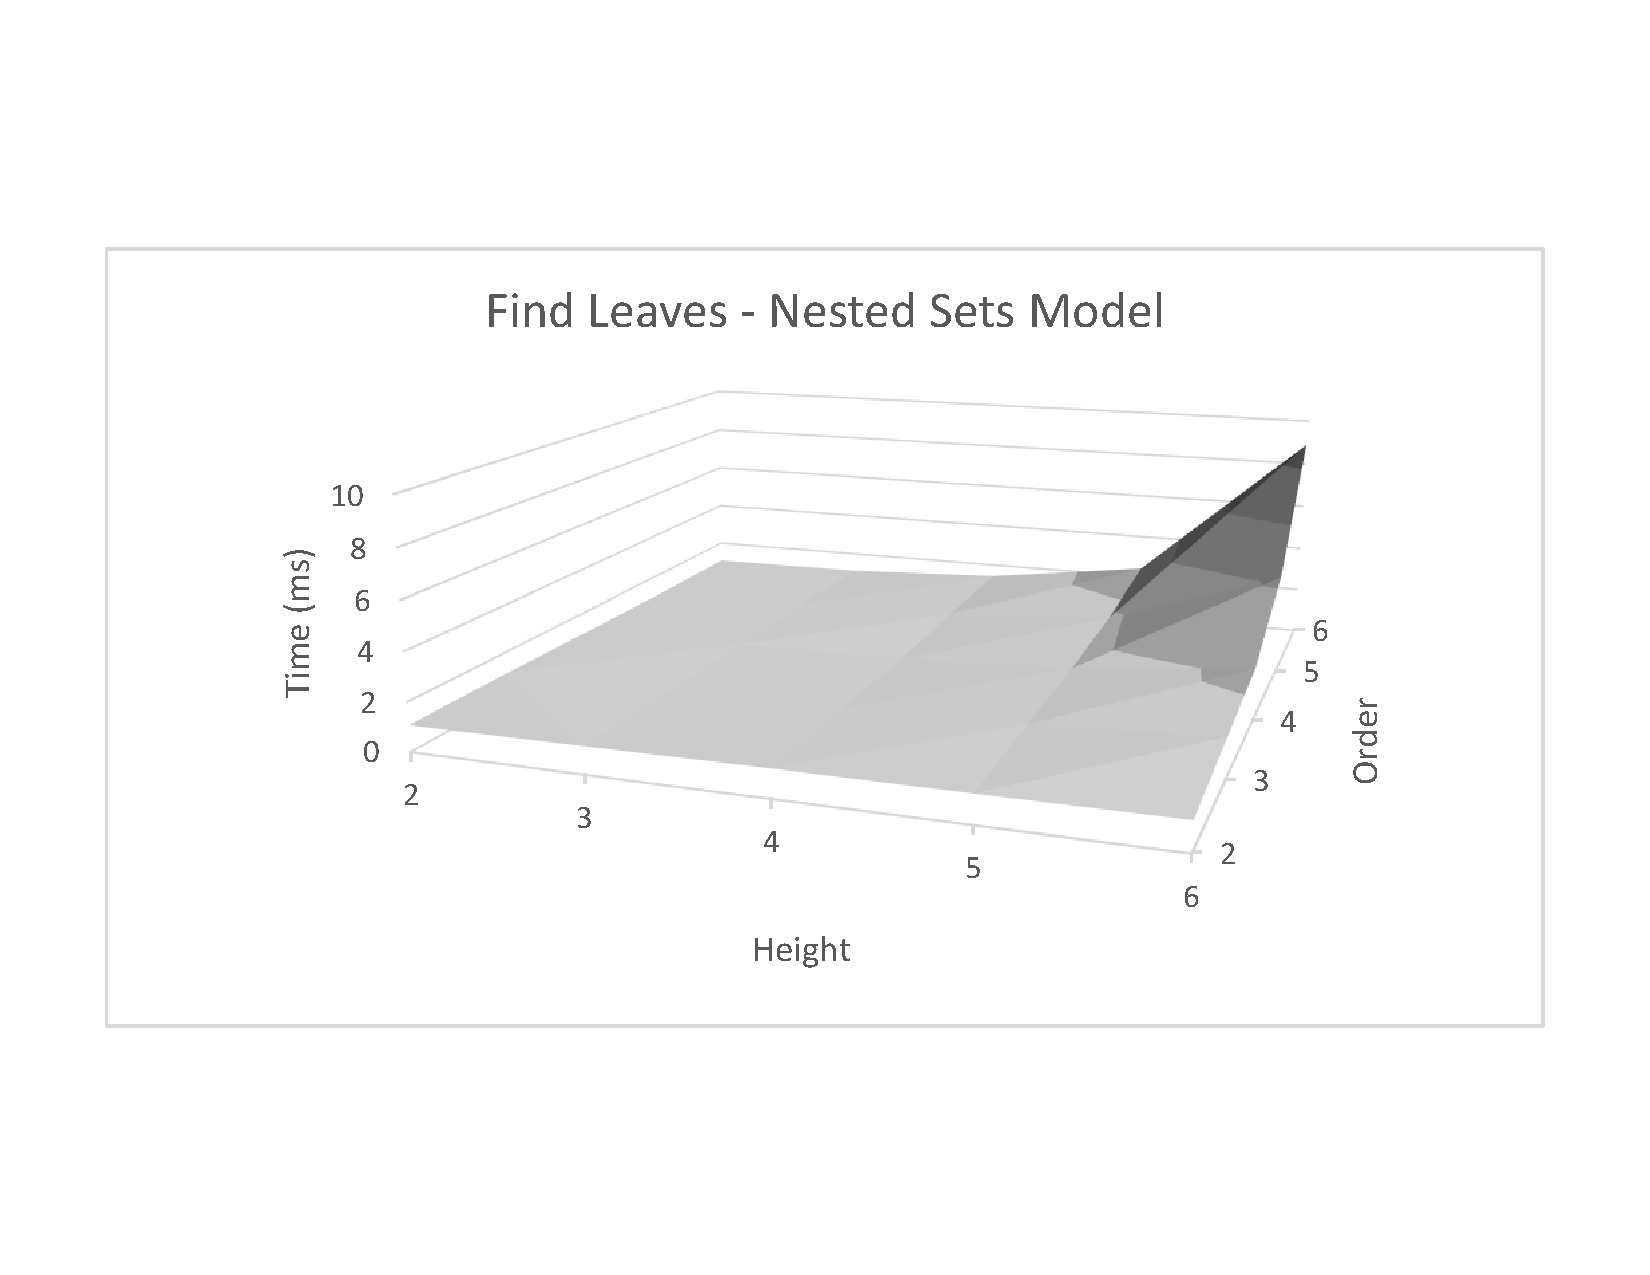
\includegraphics[width=6in]{images/eval/leaves/ns_surface.pdf}
\caption{Running time of Finding Leaves using Nested Sets Model.\label{fig-leaves-ns}}
\end{center}
\end{figure}

Figure~\ref{fig-leaves-ns} depicts the running time, in milliseconds, of the operation implemented in MySQL stored procedure. The figure has the same exponential trend as the previous two models; however, the running time using this technique is unreasonably high. For example, with height = 4 and order = 2 (N = 15), the running time is 1831 ms (almost 2 seconds) comparing with 13 ms and 1.15 ms of other two models, for very small data size. For this reason, we will no longer compare the running time of this technique to the other two.

It is interesting to reflect on this a bit. As a reminder, this technique is the Adjacency List version of the algorithm implemented in MySQL stored procedure. That means the algorithm is recursive, and we implemented a stored recursive stored procedure that is called for every node in the hierarchy. The take away here is recursive stored procedure using MySQL is possible, but it is extremely inefficient, to which we attribute this performance.

\begin{figure}[!h]
\begin{center}
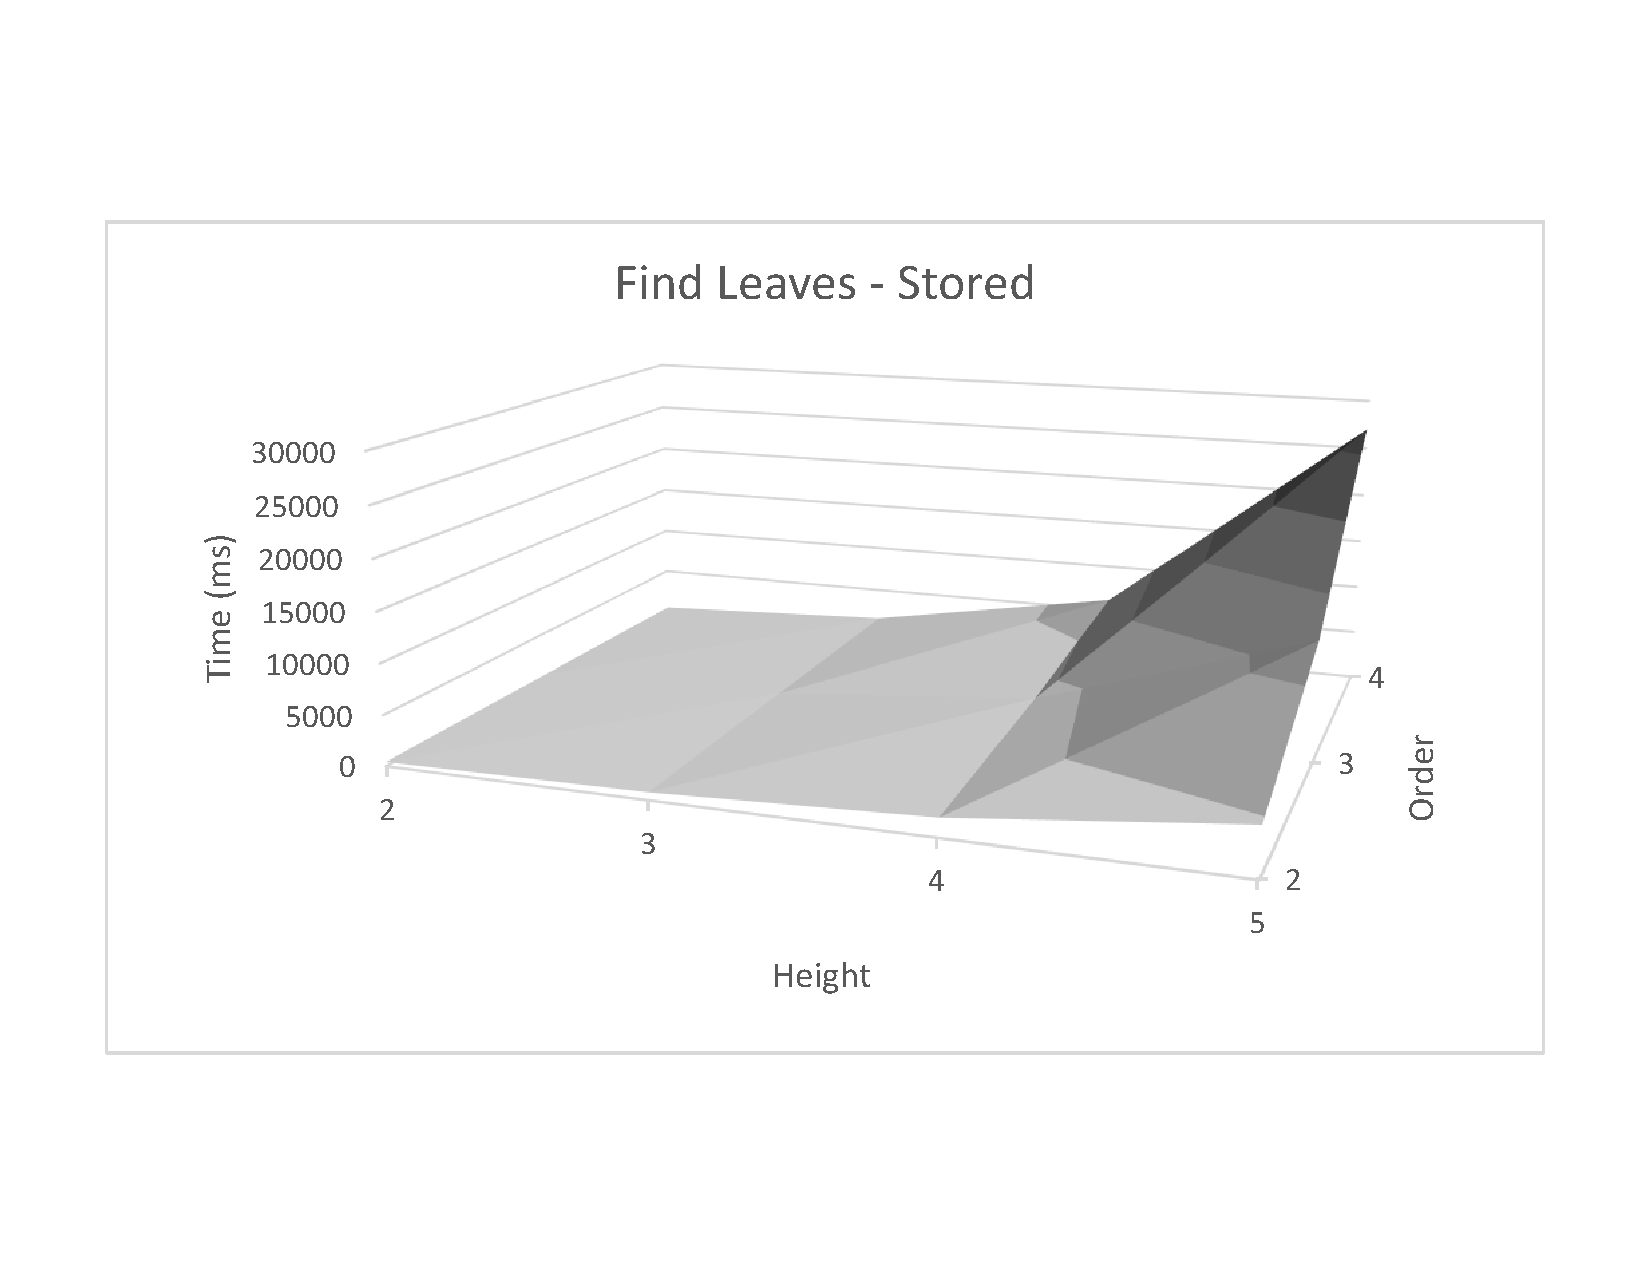
\includegraphics[width=6in]{images/eval/leaves/sr_surface.pdf}
\caption{Running time of Finding Leaves using Stored Procedure.\label{fig-leaves-sr}}
\end{center}
\end{figure}

If we take a slice of Figure~\ref{fig-leaves-al} and Figure~\ref{fig-leaves-ns} where order = 8, we can see the growth of the algorithms with respect to height, as shown in Figure~\ref{fig-leaves-height1}. One thing to note is that the numbers in this figure for Nested Sets is scaled by a factor, due to the fact that the running time for the Nested Sets Model is so much lower than that of using Adjacency List Model. We already know that the algorithm using Nested Sets is generally better; therefore the purpose of this figure is not to compare the two approach, rather is to create a model of running time for each using the data provided.


Based on the data for height = 2 to 6 as shown in previous figure, a running time growth model was build using exponential regression as shown in Figure~\ref{fig-leaves-height2}, where projections are shown in dotted lines. In addition, we use the data for height = 7 to validate our model. As shown in the figure, the projection from the growth model for the Adjacency List implementation fits the validation well. However, the model for the Nested Sets implementation grossly underestimate the value for the validation data. In this case, the running time jumped significantly since height = 7. This could be caused by that the experiment has not reached steady state at height = 6 and we need more data points to build a better model. Another reason could be, the database becomes extremely inefficient in processing the request for height higher than 6.

\begin{figure}[!h]
\begin{center}
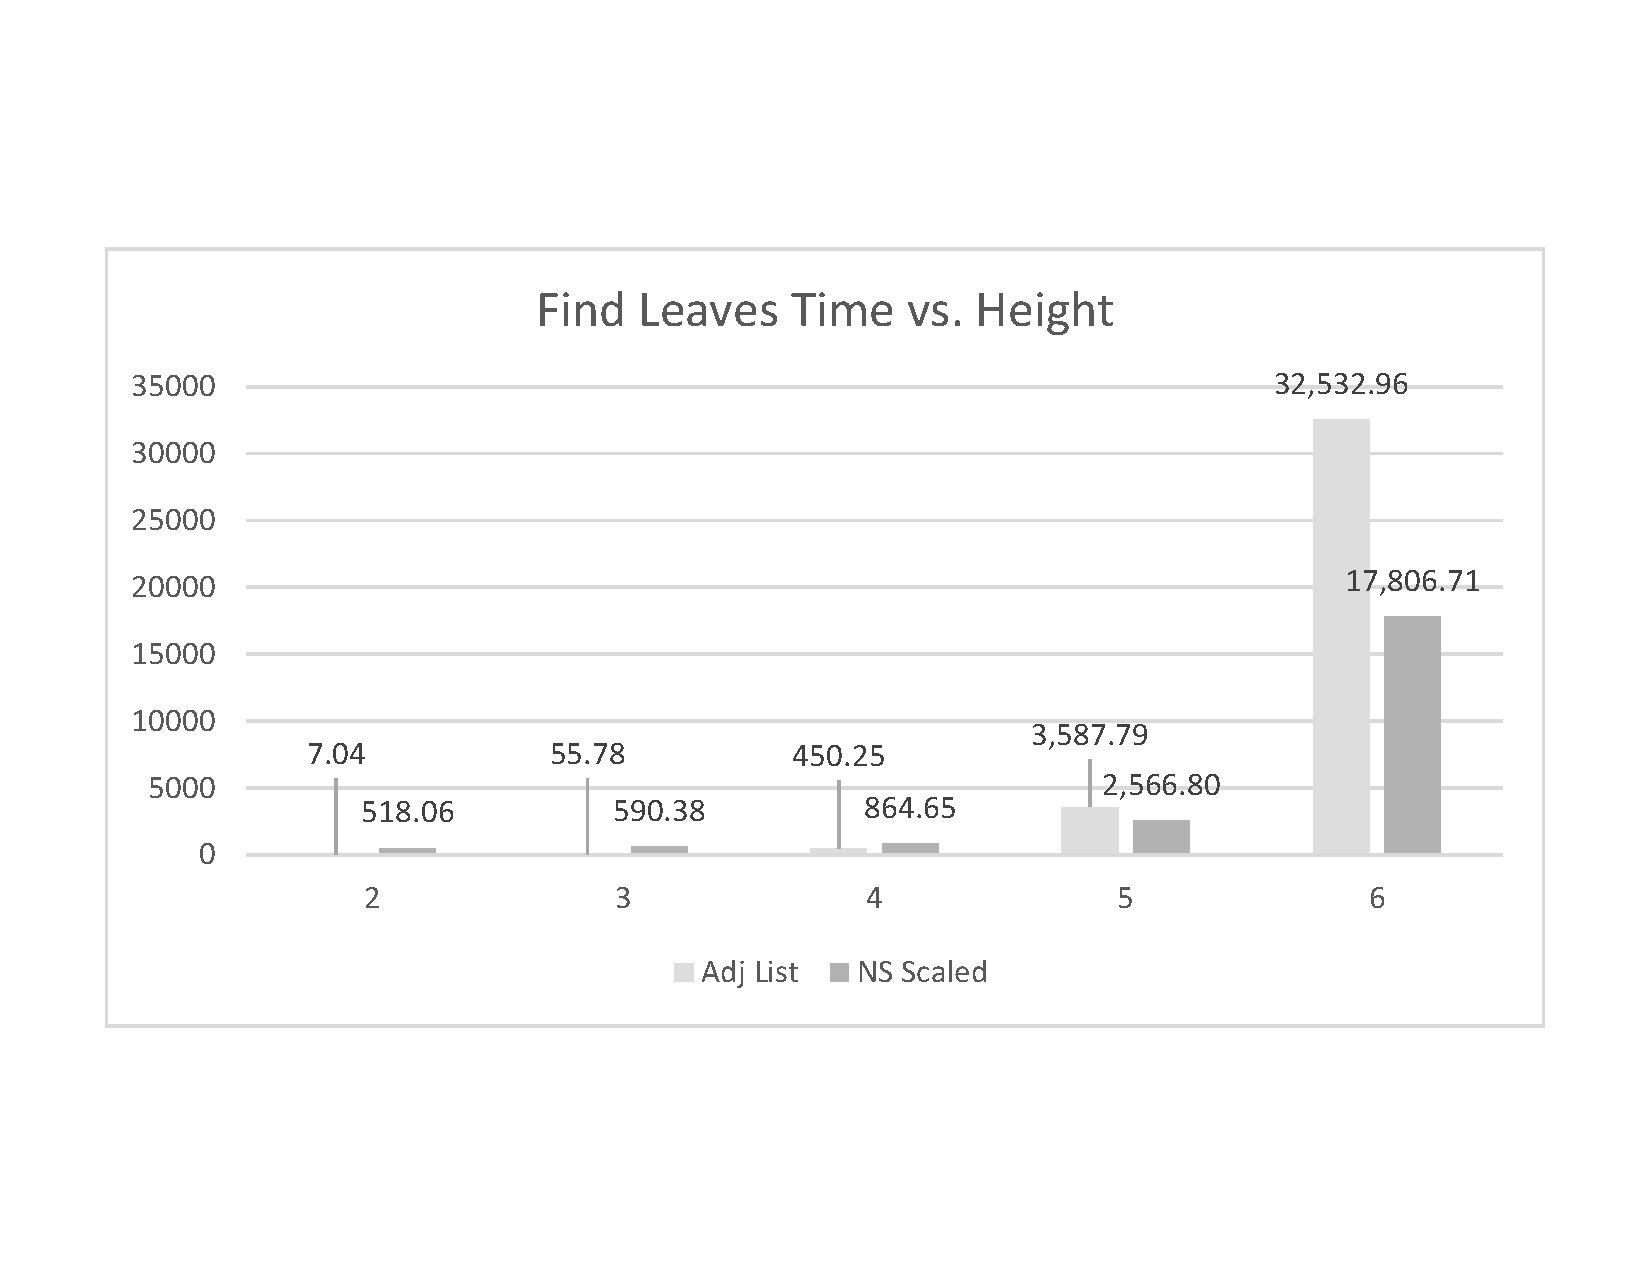
\includegraphics[width=6in]{images/eval/leaves/height/col.pdf}
\caption{Running time with respect to height at order = 8.\label{fig-leaves-height1}}
\end{center}
\end{figure}

\begin{figure}[!h]
\begin{center}
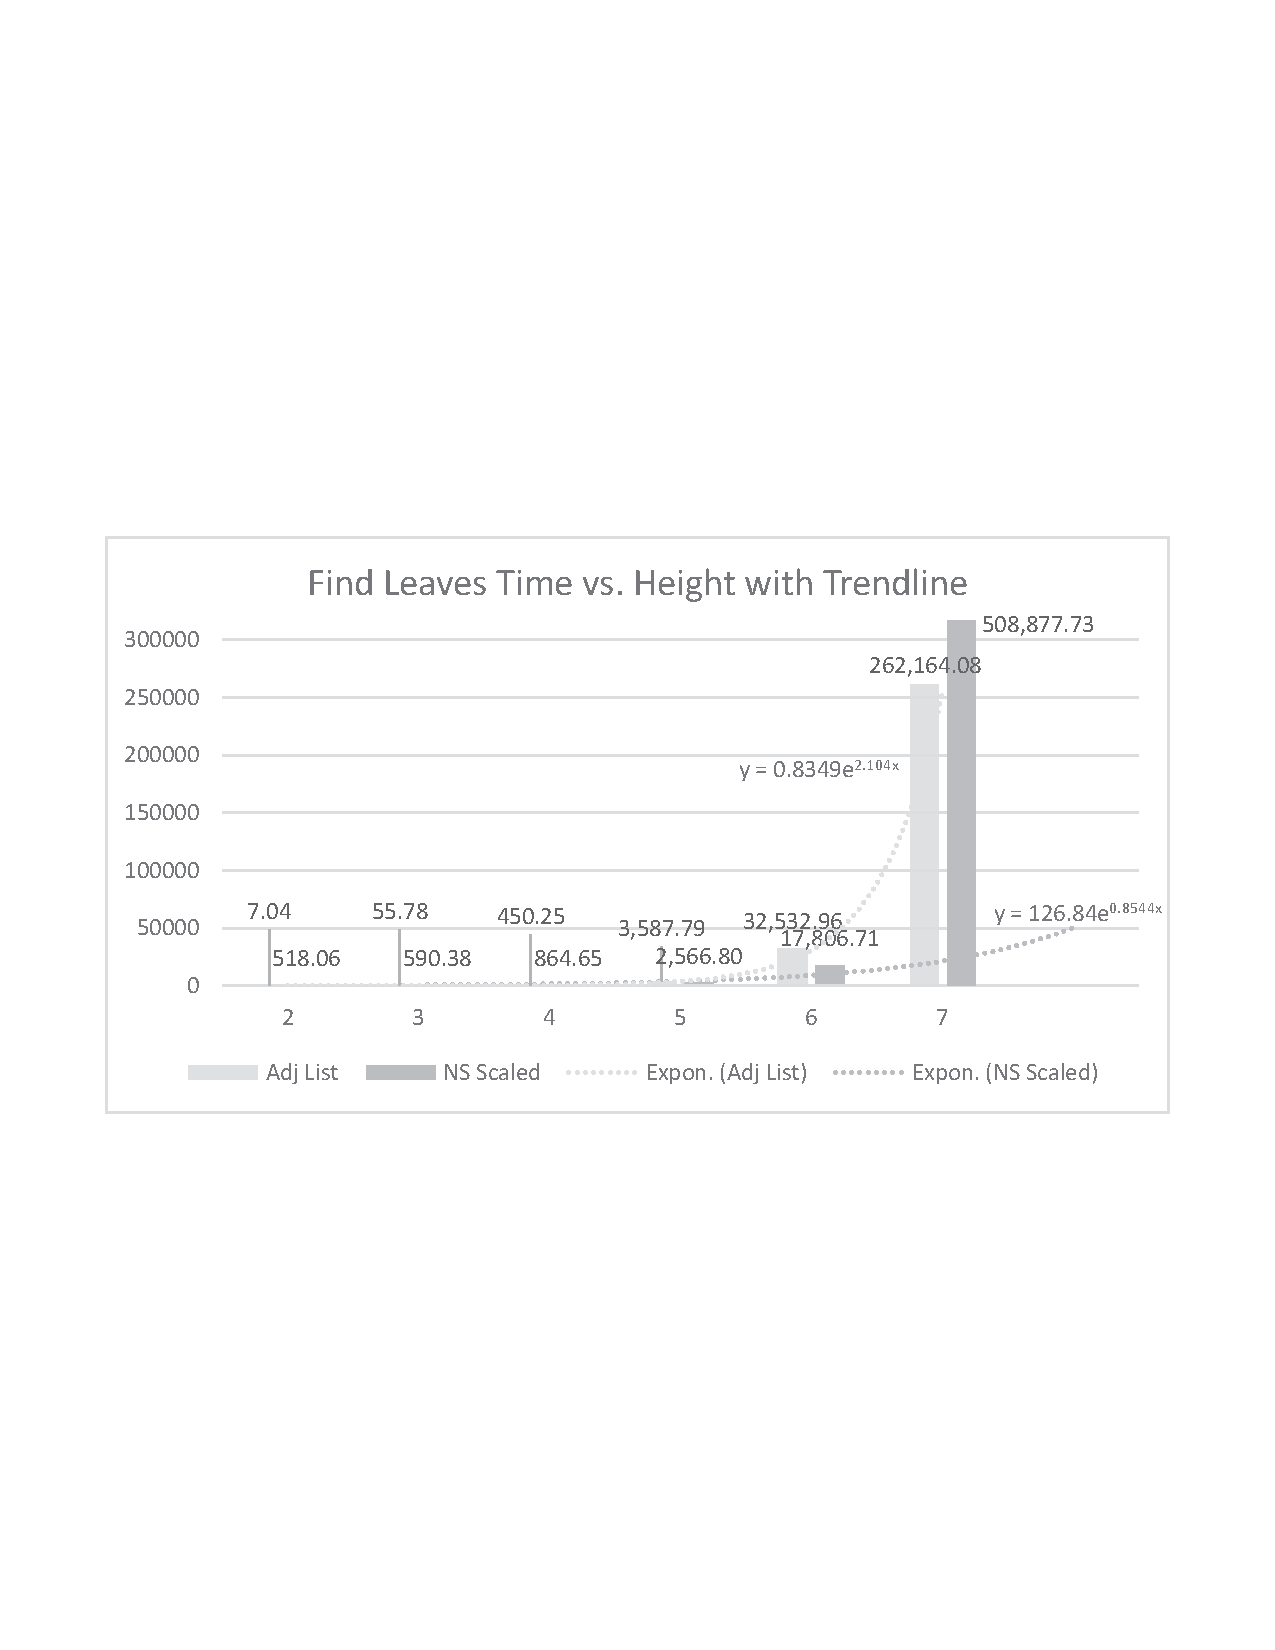
\includegraphics[width=6in]{images/eval/leaves/height/col_trend.pdf}
\caption{Running time with respect to height model at order = 8.\label{fig-leaves-height2}}
\end{center}
\end{figure}

We take the same approach to analyze the running time growth rate of the operation with respect to order and the result is shown in Figure~\ref{fig-leaves-order1} and Figure~\ref{fig-leaves-order2}. Once again, the number for Nested Sets Model in these figures are scaled to fit to combine the graph of both approaches in the same figure.

\begin{figure}[!h]
\begin{center}
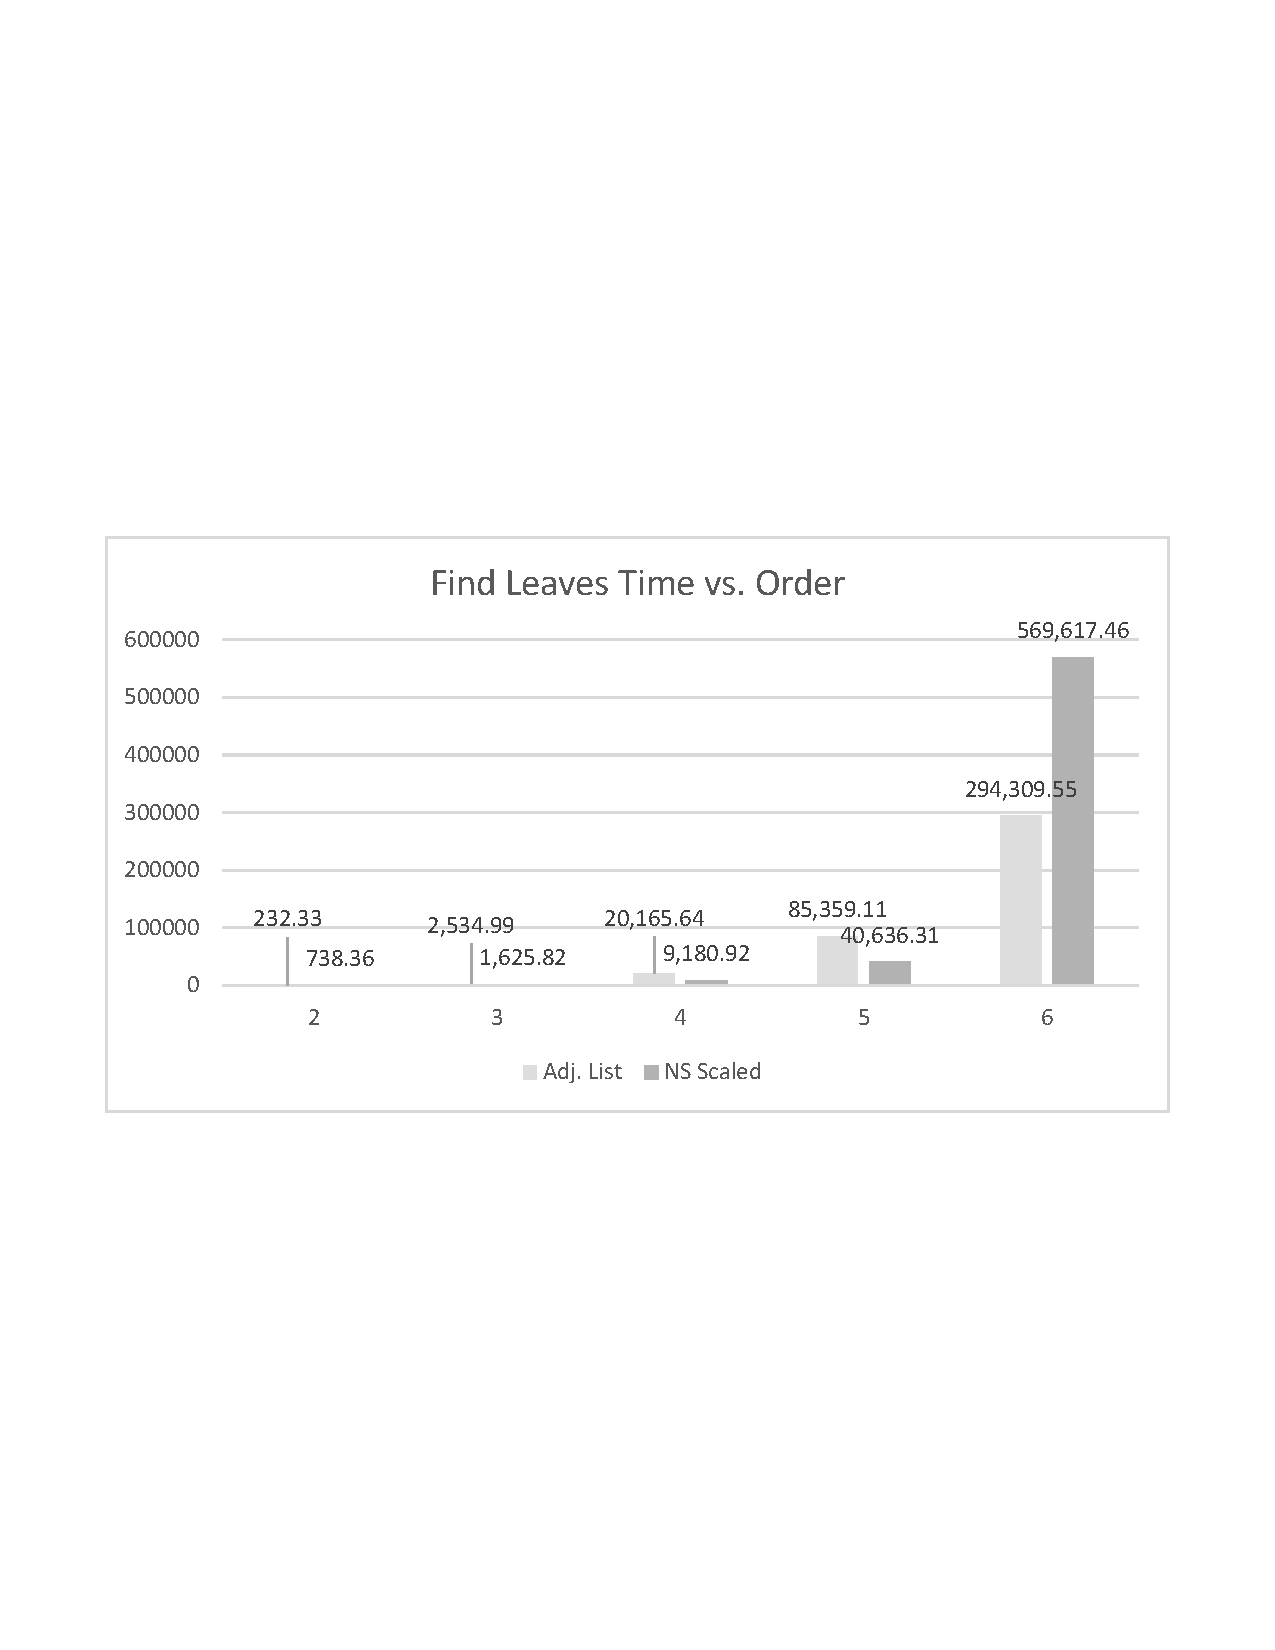
\includegraphics[width=6in]{images/eval/leaves/order/col.pdf}
\caption{Running time with respect to order at height = 8.\label{fig-leaves-order1}}
\end{center}
\end{figure}

Intuitively, the running time growth rate should grow linearly with respect to the order (or width) of the tree; however, based on the initial observation of the data, it appears to be exponential, so we build a growth rate model also using exponential regression as shown in Figure~\ref{fig-leaves-order2} and using data for order = 7 as validation for our model. As one can see from the figure, the model overestimates the running time for the Adjacency List implementation. This is an indication to confirm our intuition that the growth rate is linear instead of exponential. However, the model fits the validation well for the Nested Sets implementation. This is a bit of a surprise since, this implementation usually have better performance.

\begin{figure}[!h]
\begin{center}
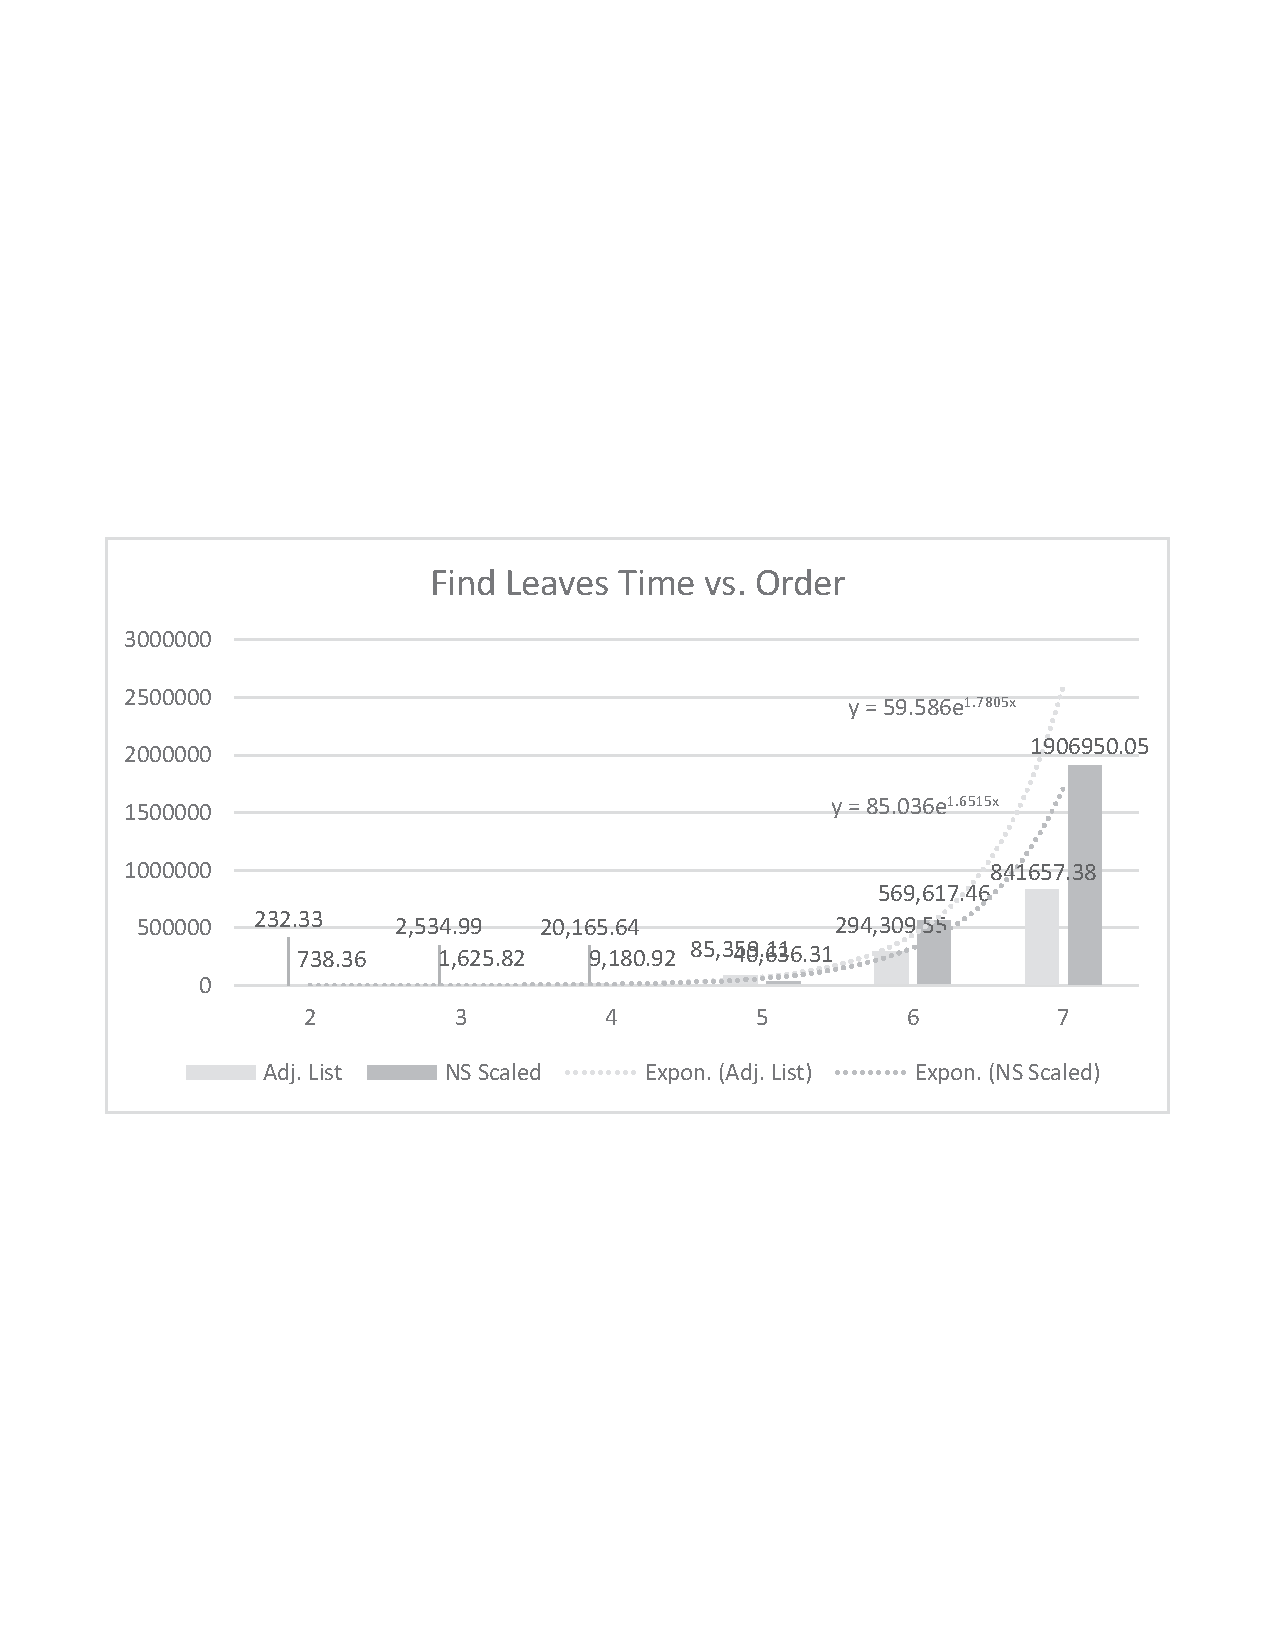
\includegraphics[width=6in]{images/eval/leaves/order/col_trend.pdf}
\caption{Running time with respect to order model at height = 8.\label{fig-leaves-order2}}
\end{center}
\end{figure}

\section{Conclusion}\label{sec_conclusion}

In this paper, we conducted performance evaluation of three implementations of hierarchy in relational database. The first is the Adjacency List Model, which is realized by storing all nodes of the hierarchy in a single Nodes table, and each node, represented by a record in the table, contains a self-referencing foreign key that references the parent node.

The second is the Nested Sets Model, which is an attempt to improve the performance of data retrieving operations over the Adjacency List Model. This model is an extension of the first in that each node (or record) contain two additional {\em left} and {\em right} fields that defines the subset relationship. Left and right fields are then indexed using B-Tree for fast access. With this extension, one can easily check if a node is in the hierarchy of another node.

The third implementation is the Stored Adjacency List, in which the same algorithm used in Adjacency List Model implemented in MySQL Stored Procedure. This technique is used to verify if stored procedure is a viable way for performance tuning for hierarchy operations.

Performance evaluation were conducted using the operations defined in Section~\ref{sec_tree_ops}. Operations are divided into 3 performance groups: O(log N), O(N), and O(1). Members of the same group have similar performance characteristic; therefore, one operation from O(log N), and O(N) is chosen for performance evaluation as representative for the group. The evaluation for group O(1) was conducted, but not reported in this paper, because the run time is negligible and not influenced by input size. The operation to find the root of a node was chosen to represent O(log N) group, and the operation to find all leaf nodes of a node was chosen to represent O(N) group. The performance of the models are measure in running time of the operations, in which the lower the running time the better.

For group O(log N), the evaluation reported in Section~\ref{eval_group1} shows the expected running time performance. For the Adjacency List Model, the growth rate of the algorithm is linear with respect to the height and constant with respect to the width (order) of the hierarchy. The Nested Sets Model is a huge improvement over the first in this evaluation. Based on the evaluation, the running time growth rate is constant for both dimensions. For the stored implementation, the running time is better than both other approaches. However, the project model is slow-growing linear with respect to height, and constant with respect to order.

In Group O(N), the Nested Sets Model still significantly outperformed Adjacency List Model; however the running time of the stored approach is unreasonable high for very small data sets. For the Adjacency List Model, the running time, as expected, have exponential running time growth with respect to the height of the tree. From the evaluation result, the growth rate with respect to width also appears to be exponential; however, our validation does not fit the exponential model, therefore we believe the growth is a steep linear model.

For the Nested Sets model, the growth rate is also exponential. Although the running times are much lower that of the other approach, the growth is faster. Frankly, I did not expect an exponential growth rate due to the optimizations that has been done. I believe this could be caused by my own implementation. As for the time complexity against the width, it is also exponential. This is also unexpected. Again this is due to that the implementation requires table joins, which degrades the performance very quickly as the data size increases.